This section describes the analysis methodology. This study uses boosted $Z\to\tauhad\taulep$ events to measure Monte Carlo correction factors for the tau identification algorithms in the high-$\pt$ region.

Different working points are defined for RNN score relative to the efficiency of selecting true $\tauhad$ candidates. When the efficiency of the working points is measured in data and simulation, a correction factor has to be derived and then applied to the simulation in order for the signal efficiency to agree between data and simulation \cite{ATLAS:2017mpa}. Because of the top quark mass, $t\bar{t}$ events are usually used as a source of high momentum taus for measuring the scale factors in the high-$p_T$ regime. However, Lepton universality may not hold in W decays. For that reason, this study uses boosted $Z\to\tauhad\taulep$ events for deriving and cross checking the simulation correction factors in the high-$p_T$ region.   
\subsection{Signal Events}\label{signalevents}
For this study, we consider as signal the events where one the taus decays hadronically and the other leptonically, either into an electron or a muon. Thus, our final states will include a $\tauhad$ candidate and one light lepton $l=e,\mu$. The presence of the light lepton will be used as our tag. 
Generally, in $Z\to\tau\tau$ events, the taus are produced back to back and their $\pt$ spectrum falls sharply. In order to select boosted taus, we look for events where the opening angle in the transverse plane between the taus ($\Delta\phi(\tauhad,\taulep)$) is narrower than usual. A depiction of the topologies of our signal events is shown in Fig.\ref{Fig1}. For these events, the missing transverse momentum ($\met$) is assumed to come from the neutrinos produced in the decays of the tau leptons. Due to the fact that two neutrinos are produced in the leptonic decay mode we expect our events to have a larger $\met$ component along the $\taulep$ direction.
\begin{figure}[htbp]
	\centering
	\subfloat[]{\label{Fig1a}{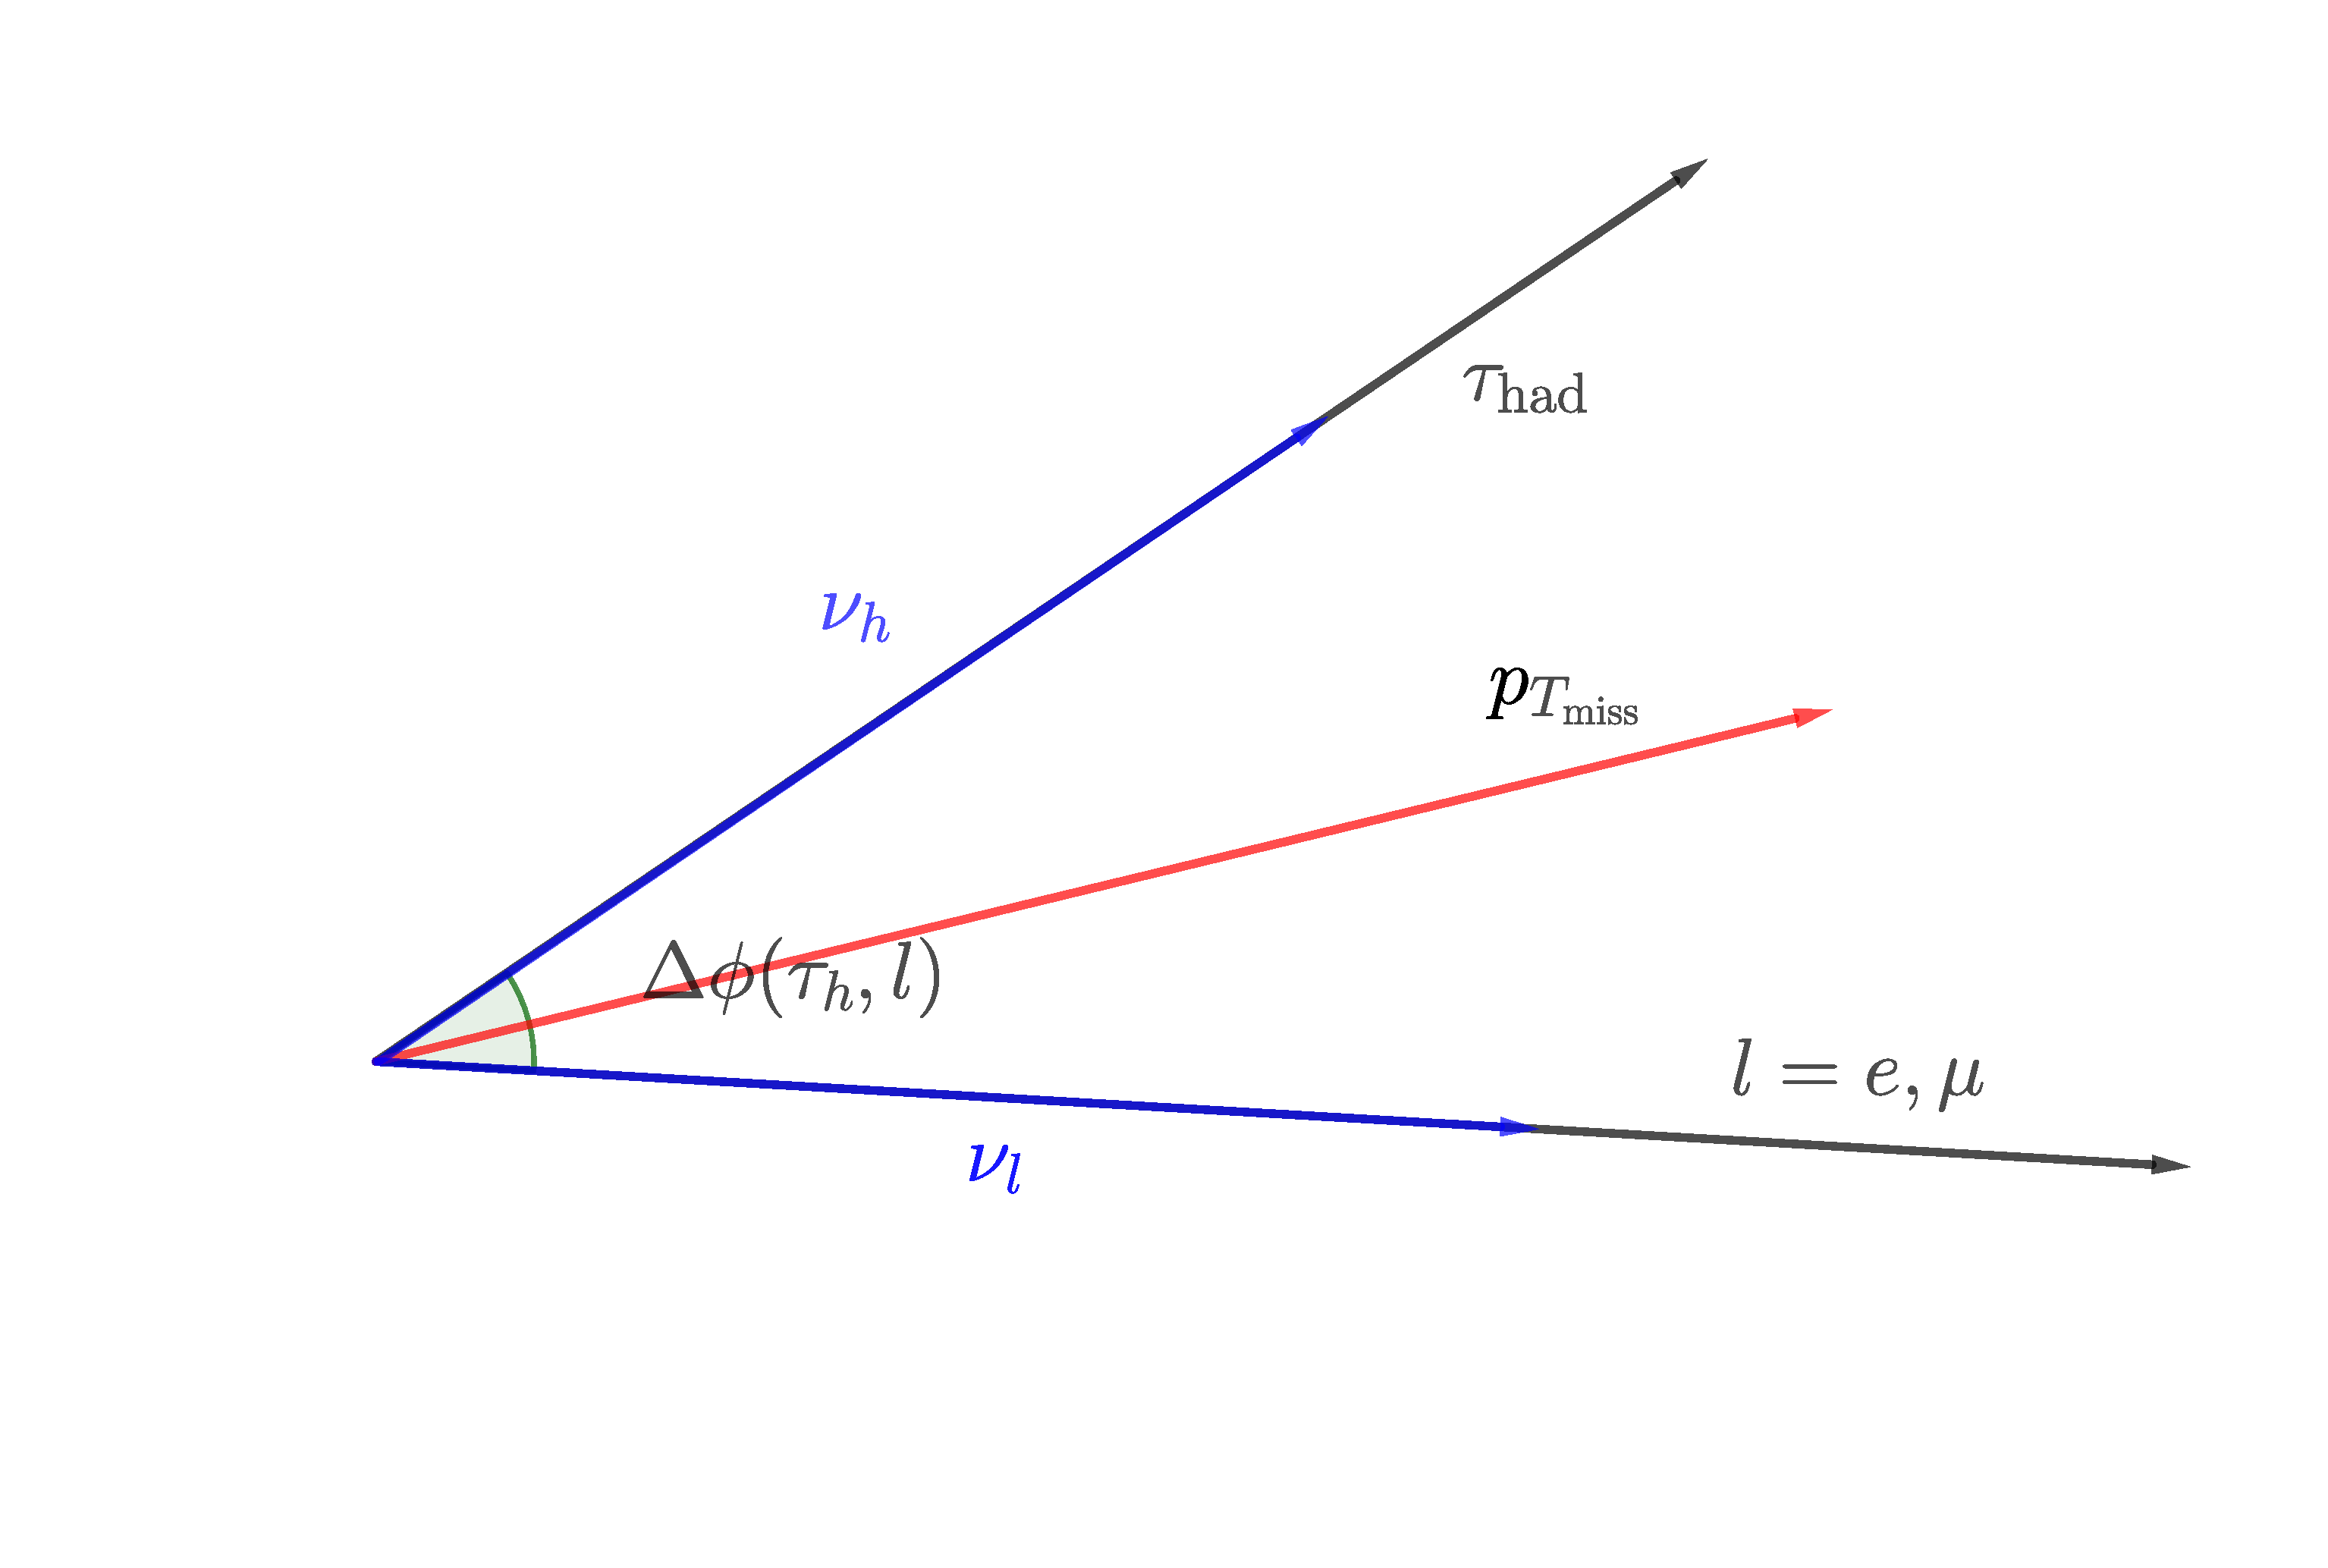
\includegraphics[width=0.49\textwidth]{Fig1a}}}\hfill
	\subfloat[]{\label{Fig1b}{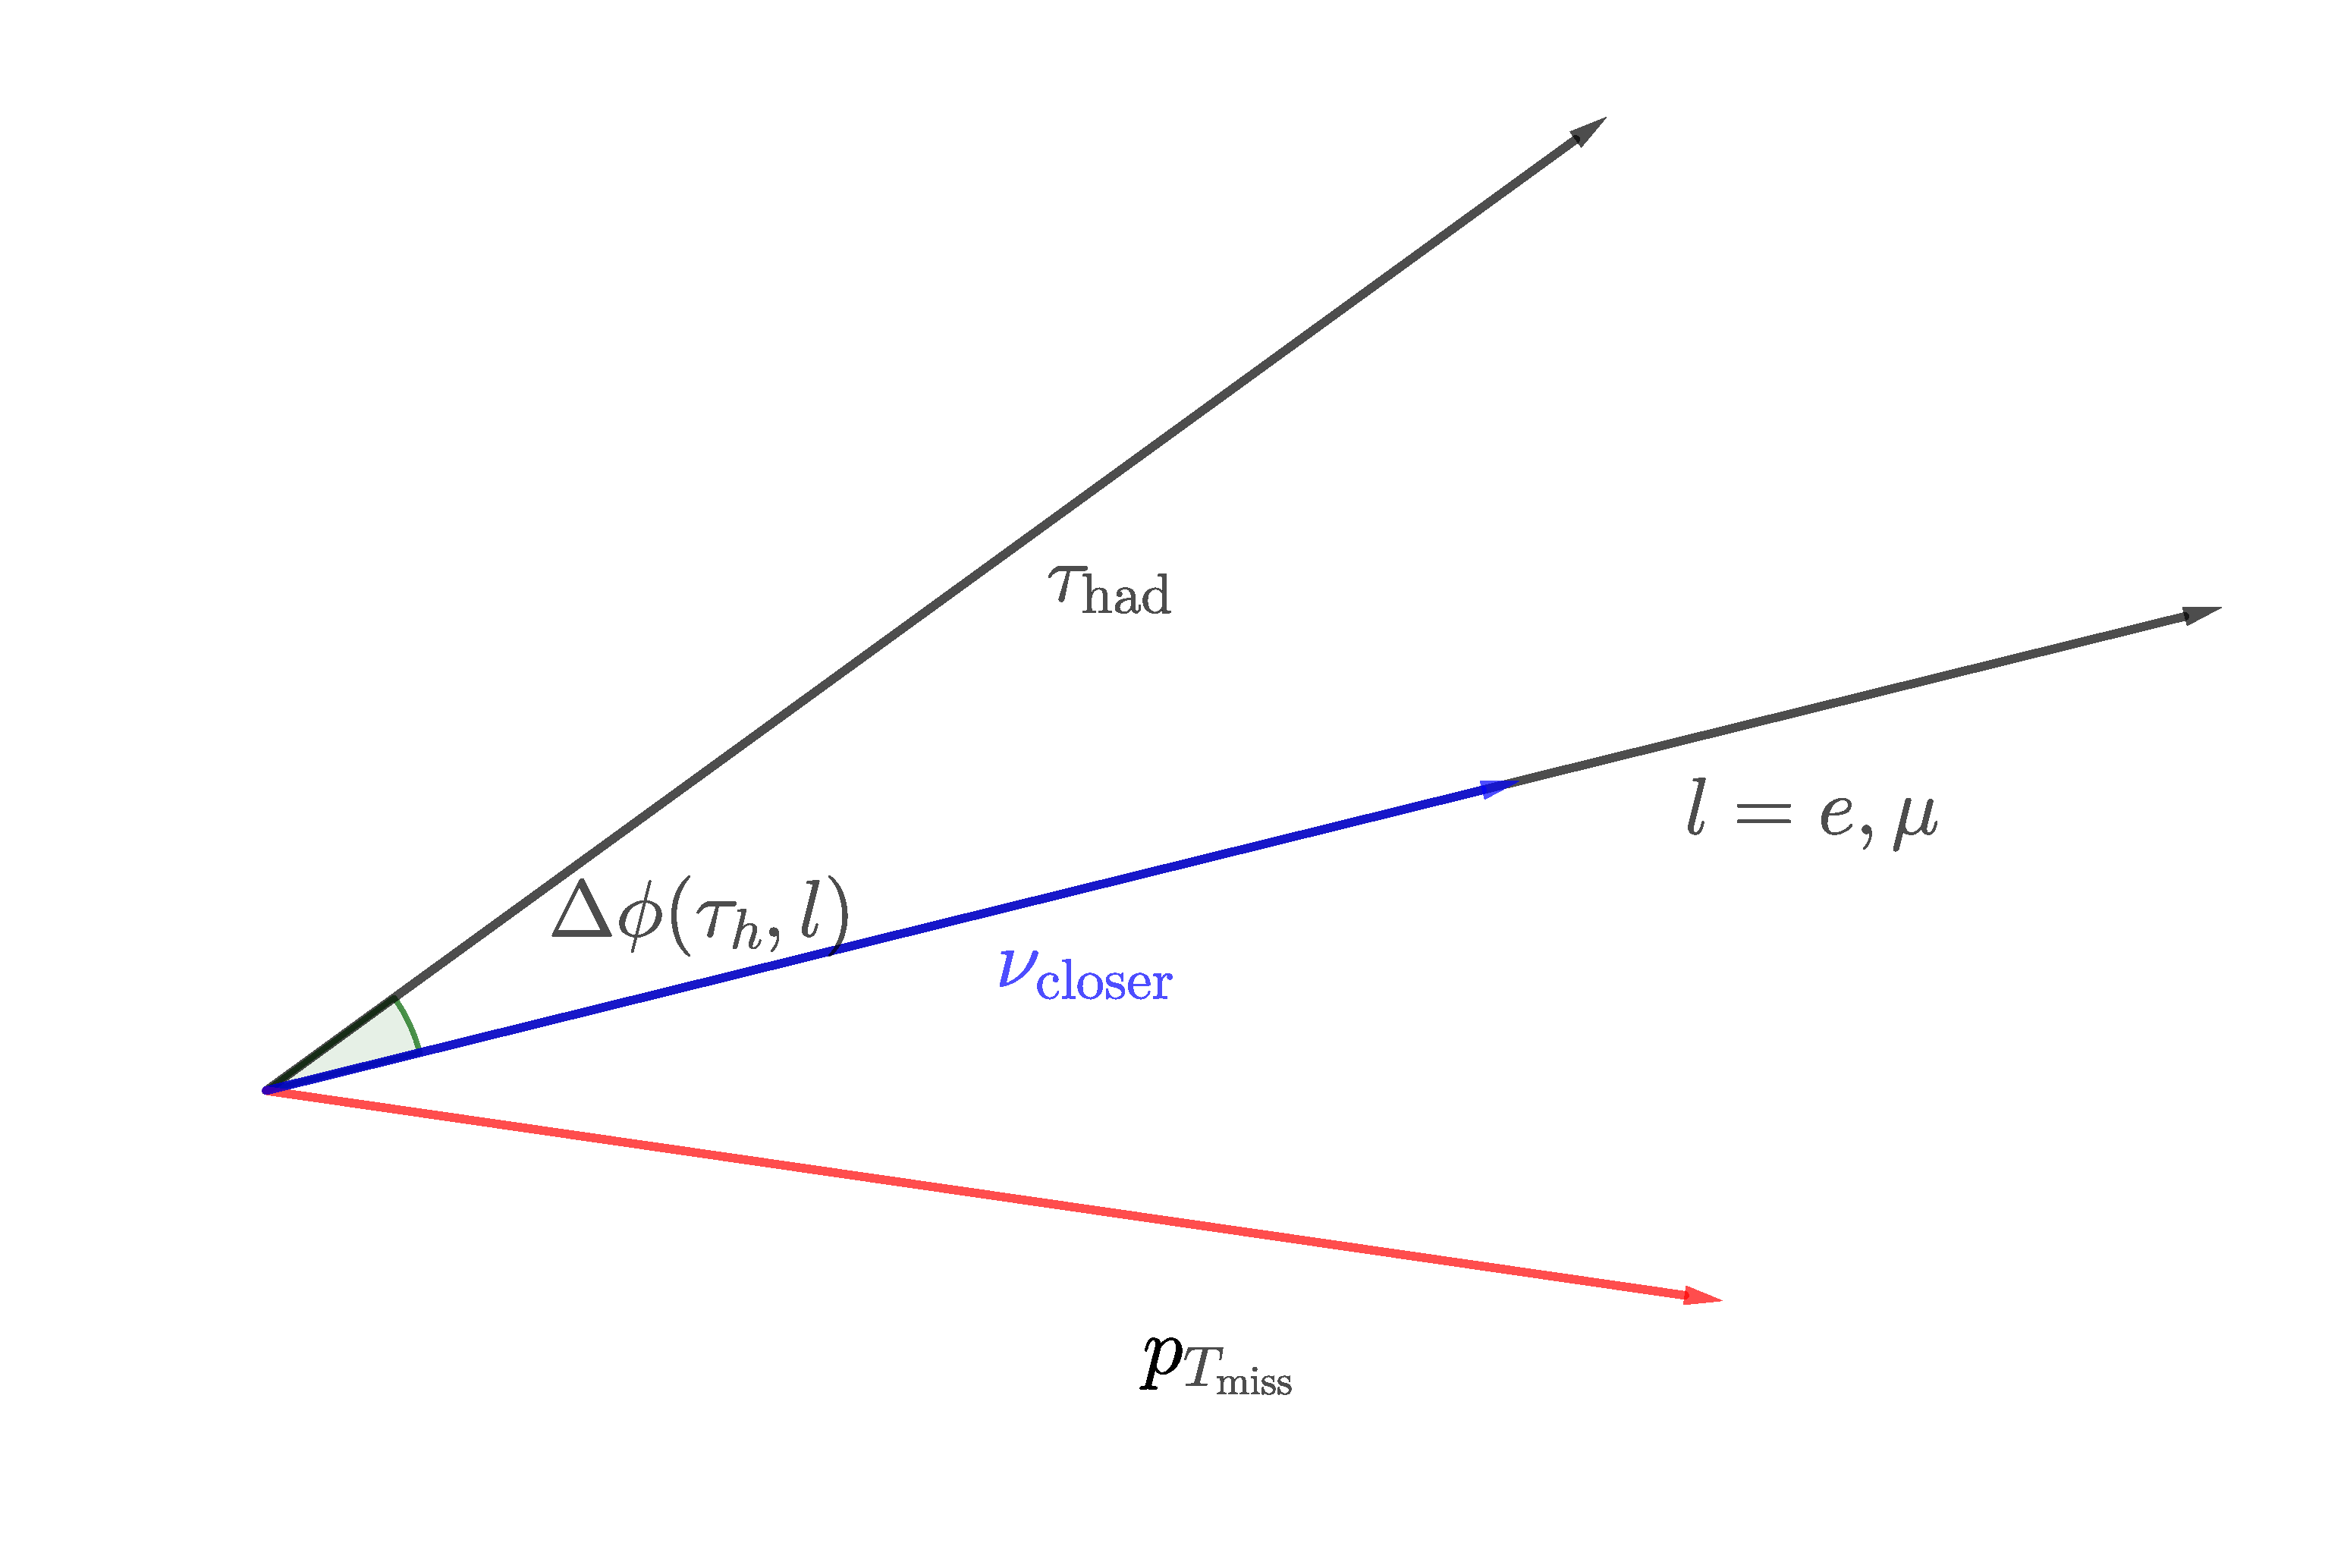
\includegraphics[width=0.49\textwidth]{Fig1b}}}
	\caption{The two different types of topologies that define the signal events. On the left, when the missing energy is between the visible objects. For these events two neutrinos are assumed to be responsible for all the missing energy. On the right, when the missing energy is outside only one neutrino is assumed to be flying on the direction of the visible object closest to the missing energy.}
	\label{Fig1}
\end{figure}

Events are classified into two topologies. First, the events where the $\met$ is inside the opening angle between the visible objects. For this kind of events, we assume that the missing energy is due to a pair of neutrinos flying in the same direction as the visible objects. This is shown in Fig.\ref{Fig1a}. In this case, the following equation is solved to obtain the momentum of the neutrinos:
\begin{equation}
\vec{p}_{T_{\nu_l}}+\vec{p}_{\nu_h}=\vec{\met},
\end{equation}
given the following set of constraints (\textit{collinear approximation}):
\begin{align}
	\phi(\nu_l)&=\phi(l),
	\\
	\phi(\nu_h)&=\phi(\tauhad),
	\\
	\eta(\nu_l)&=\eta(l),
	\\
	\eta(\nu_h)&=\eta(\tauhad).
\end{align}
In the second case, when the $\met$ is pointing outside the angle formed by the visible objects, the assumption is that only one neutrino is responsible for the majority of the $\met$. We suppose the neutrino is flying in the direction of the visible object that is closest to the $\met$, as is shown in Fig.\ref{Fig1b}. The following equations are used to obtain the neutrino momentum:
\begin{align}
	p_{T_{\nu}}&=\met \cos(\Delta\phi(\tau_{\text{closer}},\met)),
	\\
	\phi(\nu)&=\phi(\tau_{\text{closer}}),
	\\
	\eta(\nu)&=\eta(\tau_{\text{closer}}),
\end{align} 
where $\tau_{closer}$ stands for the visible object closest to the direction of the $\met$.

A variable called $\Omega$ is defined in order to classify the events in one of the described topologies . First, we define:
\begin{equation}
\omega=\frac{\Delta\phi(\tau_{\text{closer}},\met)}{\Delta\phi(\tauhad,\taulep)},
\end{equation}
then,
\begin{itemize}
	\item when $\met$ is inside the opening angle between the visible objects but closer to $\tauhad$:
	\begin{equation}
	\Omega=\omega,
	\end{equation}
	\item when $\met$ is still inside, but closer to $\taulep$:
	\begin{equation}
	\Omega=1-\omega.
	\end{equation}
	\item If $\met$ is outside and closer to $\tauhad$:
	\begin{equation}
	\Omega=-\omega,
	\end{equation}
	\item and finally, if $\met$ is outside and closer to $\taulep$:
	\begin{equation}
	\Omega=\omega+1.
	\end{equation}
\end{itemize}
Thus, $\Omega$ is a continuous variable that gives information on the topology of the event. When the $\met$ is inside the visible system it has values in the interval [0,1]. It is exactly zero when $\met$ is in the $\tauhad$ direction and one when $\met$ is in the $\taulep$ direction. $\Omega$ has negative values when the $\met$ is outside and closer to the $\tauhad$ candidate and has positive and values greater than one when is outside and closer to the $\taulep$. A diagram describing the $\Omega$ values is shown in Fig.\ref{Fig2}.
\begin{figure}[htbp]
	\centering
	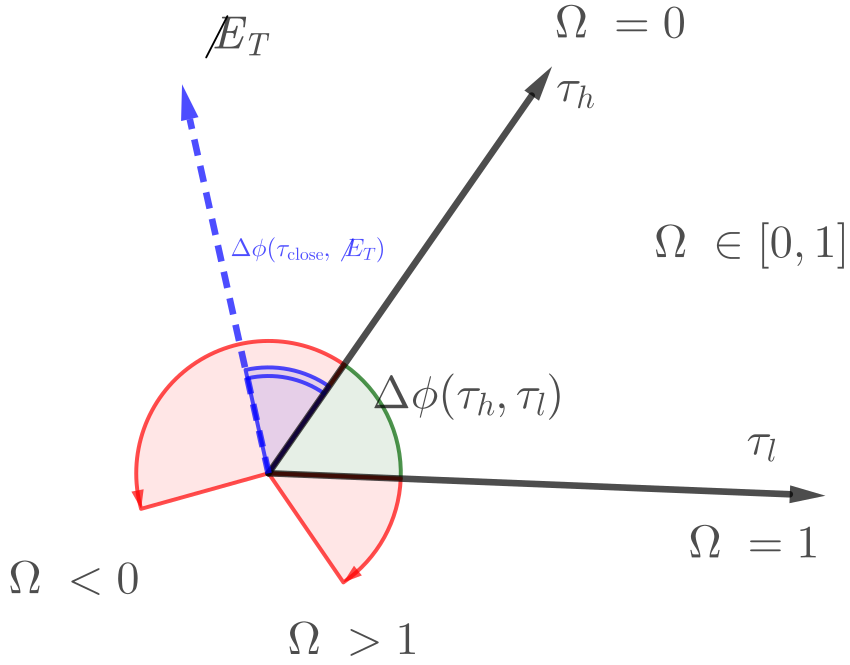
\includegraphics[width=0.5\textwidth]{Fig2.png}
	\caption{Graphical representation of the different values of $\Omega$ depending on the region where the $\met$ is located.}
	\label{Fig2}
\end{figure}
As we will see later, the event classification into these different topologies will allow us to reconstruct and exploit kinematic variables as the invariant mass of the di-tau system, the Z boson transverse momentum ($Z\pt$) and the angular distribution of the objects in the event.

\subsection{Scale Factors Calculation}\label{sec3.2}
Conventionally, the correction or scale factors (SFs), are defined as the ratio of the efficiency in data and simulation of a $\tauhad$ candidate to pass a certain level of identification. The main challenge in that approach is the estimation of the background coming from QCD initiated jets. Additionally, $\POWPY$ and $\SHERPA$ simulations give different predictions for the $Z\pt$. Consequently, distinct MC generators will predict different kinematics for the reconstructed objects and this will affect the measurement.

For this measurement, an alternative approach has been taken. First, the ratio of observed signal events to predicted events in simulation for $Z\to\tauhad\taulep$ is defined as:
\begin{equation}
	C_{X}(Z\to\tauhad\taulep)=\frac{\NData}{\NMC}.
	\label{eq14}
\end{equation}
Where X is any of the tau-ID working points, $\NData$ is the number of $Z\to\tauhad\taulep$ events observed in the data having subtracted the background predictions and $\NMC$ are the number of simulated $\Ztt$ events with one truth-matched $\tauhad$. Next, we calculate the same ratio but for $Z\to ll$ events:
\begin{equation}
C(Z\to ll)=\frac{\NData}{\NMC}.
\end{equation}
Here, $\NData$ is the number of $Z\to ll$ events observed in data having subtracted the background predictions and $\NMC$ is the number of simulated $\Zll$ events passing all the selections.

Finally, to define the SFs we take the following double ratio:
\begin{equation}
SF_{X}=\frac{C_{X}(Z\to\tauhad\taulep)}{C(Z\to ll)}.
\end{equation}
With this method, at first order, it is expected that some of the light lepton related uncertainties cancel. Additionally, phenomenological and luminosity uncertainties would be reduced as well.

However, it is important to point out that this method does not have some of the advantages offered by the traditional measurement. In that case, it is the efficiency itself what is compared between data and MC. This helps to partially cancel the systematic uncertainties, coming for instance, from the calibration of the $\pt$ of the taus. This happens since both in the numerator and denominator the MC yields are affected by the tau calibration systematics.
  
\subsection{Event Selection}\label{sec3.3}
\subsubsection{$Z\to\tauhad\taulep$ Events}\label{sec3.3.1}
In order to select $Z\to\tauhad\taulep$ events, the basic selection includes events with exactly one light lepton and one or more loose $\tauhad$ candidates. The $\tauhad$ and lepton pair need to have opposite charge. The presence of the lepton will be used as our tag, thus, a lepton trigger is required to be fired with an online requirement on the $p_{T}(\mu)\geq 20$ ($p_{T}(e)\geq 24$) GeV for 2015 data taking period. For 2016-2018 the online requirement is $p_{T}(\mu,e)\geq 26$ GeV. The muon is required to pass a \textit{medium} ID requirement and the electron has to pass a \textit{tight} ID filter. Additionally, both muons and electrons have to pass an offline $p_T$ requirement, it has to be greater than 27 GeV. Finally, the opening angle between the two visible objects $\Delta\phi(\tauhad,l)\leq 1.0$ rad.

Events containing b-jets are vetoed to reject $t\bar{t}$ background. In addition, an isolation criterion is required to be passed by the leptons: for the muon (electron), the scalar sum of the $p_T$ of the tracks within a cone of $\Delta R=0.3 (0.2)$ of the muon (electron) must be less than 0.06 times the muon (electron) $p_T$. Additionally, for the electron, the sum of the calorimeter cluster energy in a cone of size $\Delta R=0.2$ must be 0.06 times smaller than the electron $p_T$. As discussed above, we expect signal events to peak around $\Omega=1$, thus we select events where $\Omega\in (-0.2,1.6)$. Fig.\ref{Fig3} shows the $\Omega$ distribution for the $Z\to\tauhad\mu$ final state.
\begin{figure}[htbp]
	\centering
	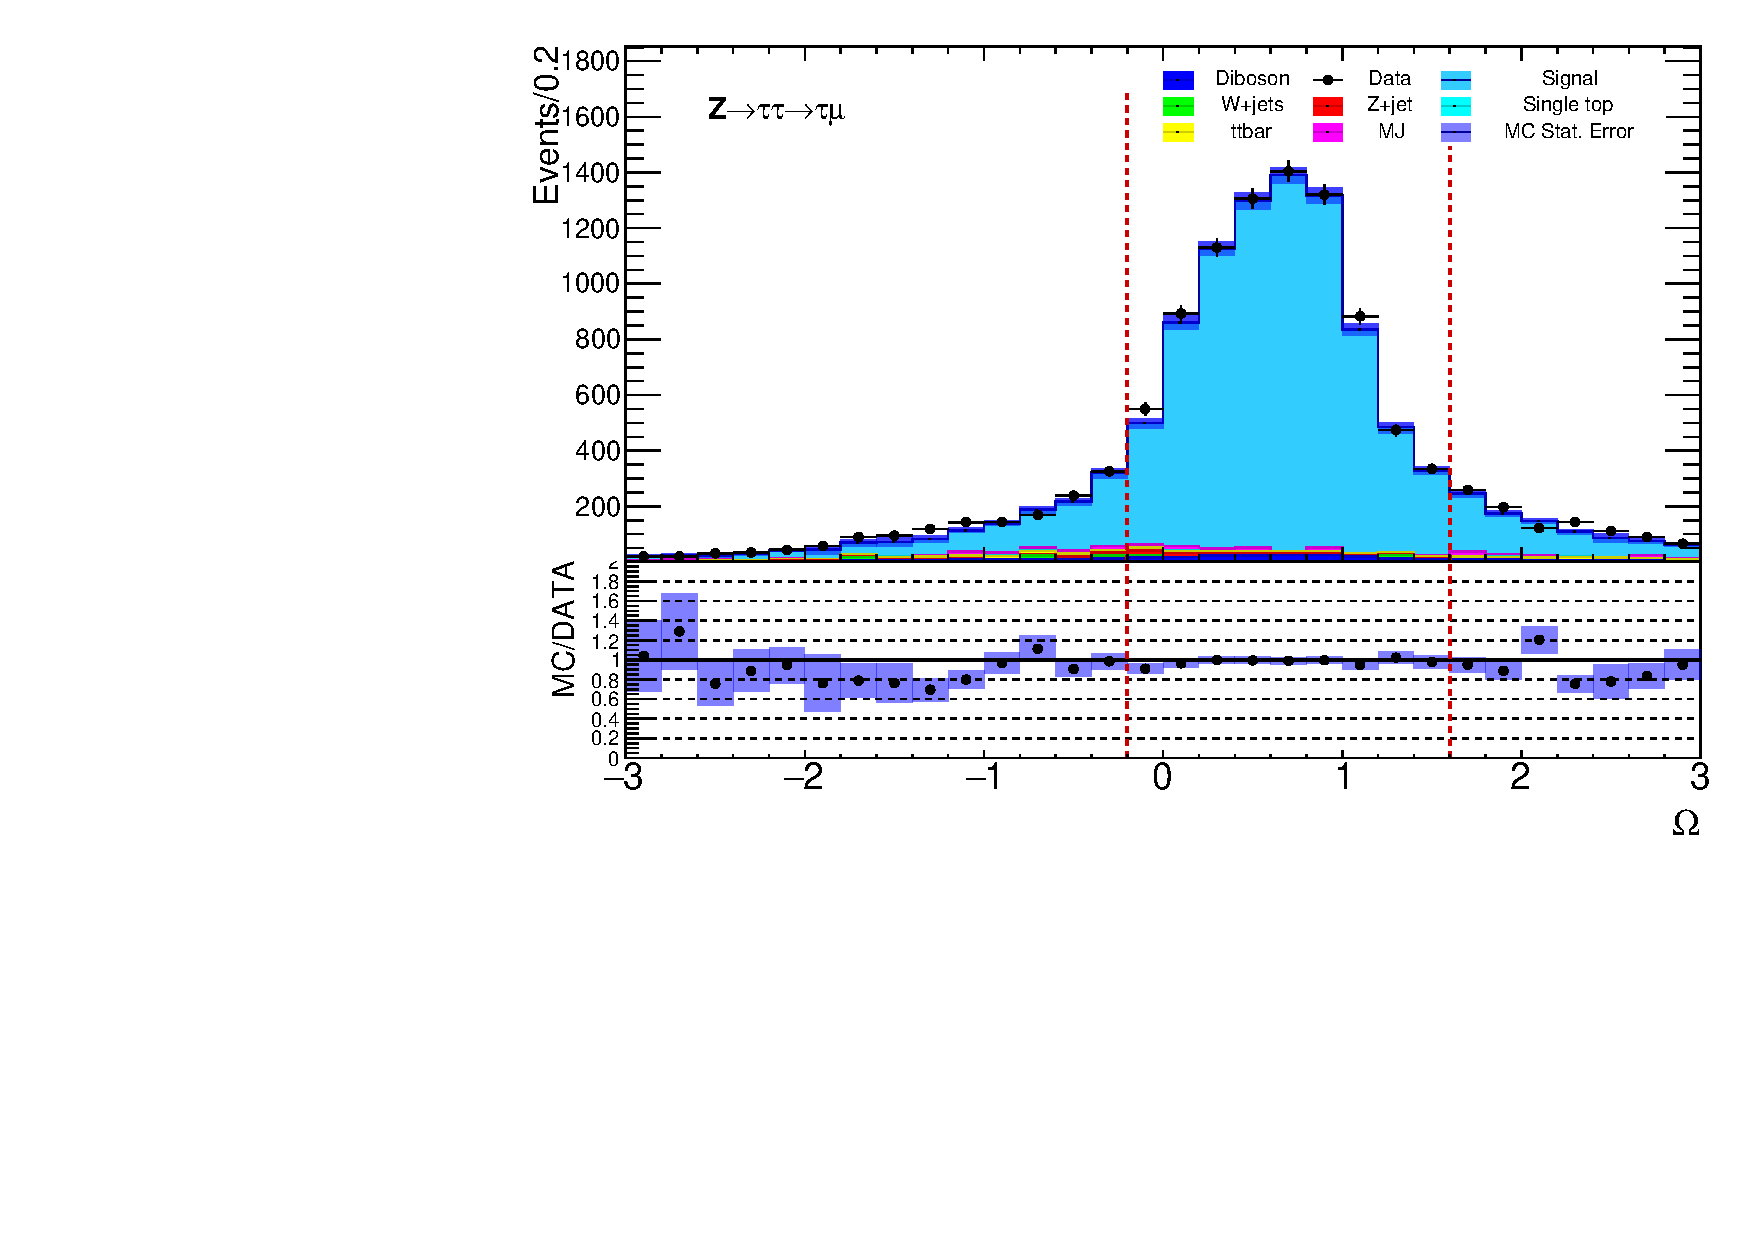
\includegraphics[width=0.6\textwidth]{figures/Fig3.pdf}
	\caption{Distribution of $\Omega$ for the $Z\to\tauhad\mu$ final state. All the other cuts have been applied apart from the one being plotted. The ATLAS data is shown as points with error bars, showing the statistical uncertainties. The detector-level predictions are shown as the coloured histograms, with the colour code as given on the plots.The region between the vertical dashed red lines is included in the final event selection. The lower section of each plot shows the ratio of prediction to data. The uncertainties on the predictions represent the MC statistical uncertainties. These uncertainties are shown as the blue shaded regions.}
	\label{Fig3}
\end{figure}
Additionally, a cut on the reconstructed invariant mass ($\mreco$) of the event is made. The cut is designed to pick events where the invariant mass is around the Z boson mass ($60\leq\mreco\leq 120$ GeV). The invariant mass of the final states is calculated depending on the event topology. For events where $\Omega\in [0,1]$ (\textit{in-between events}),
\begin{equation}
\mreco^{2}=(q_l+q_{\tauhad}+q_{\nu_l}+q_{\nu_{\tauhad}})^2.
\label{eq35a}
\end{equation}
When the $\met$ is outside (\textit{outside events}),
\begin{equation}
(\mreco-5)^{2}=(q_l+q_{\tauhad}+q_\nu)^2.
\label{eq35b}
\end{equation}
The RHS of \eqref{eq35a} and \eqref{eq35b} are 4-vector sums, where $q$ represents the four-momentum of each particle. In the outside events case we manually add 5 GeV, since in this region we find empirically that the di-tau mass is underestimated and we wish to apply the same selection in both regions. Fig.\ref{Fig4} shows the distribution of $\mreco$ for the in-between and outside $Z\to\tauhad\mu$ events. 
\begin{figure}[htbp]
	\centering
	\subfloat[]{\label{Fig4a}{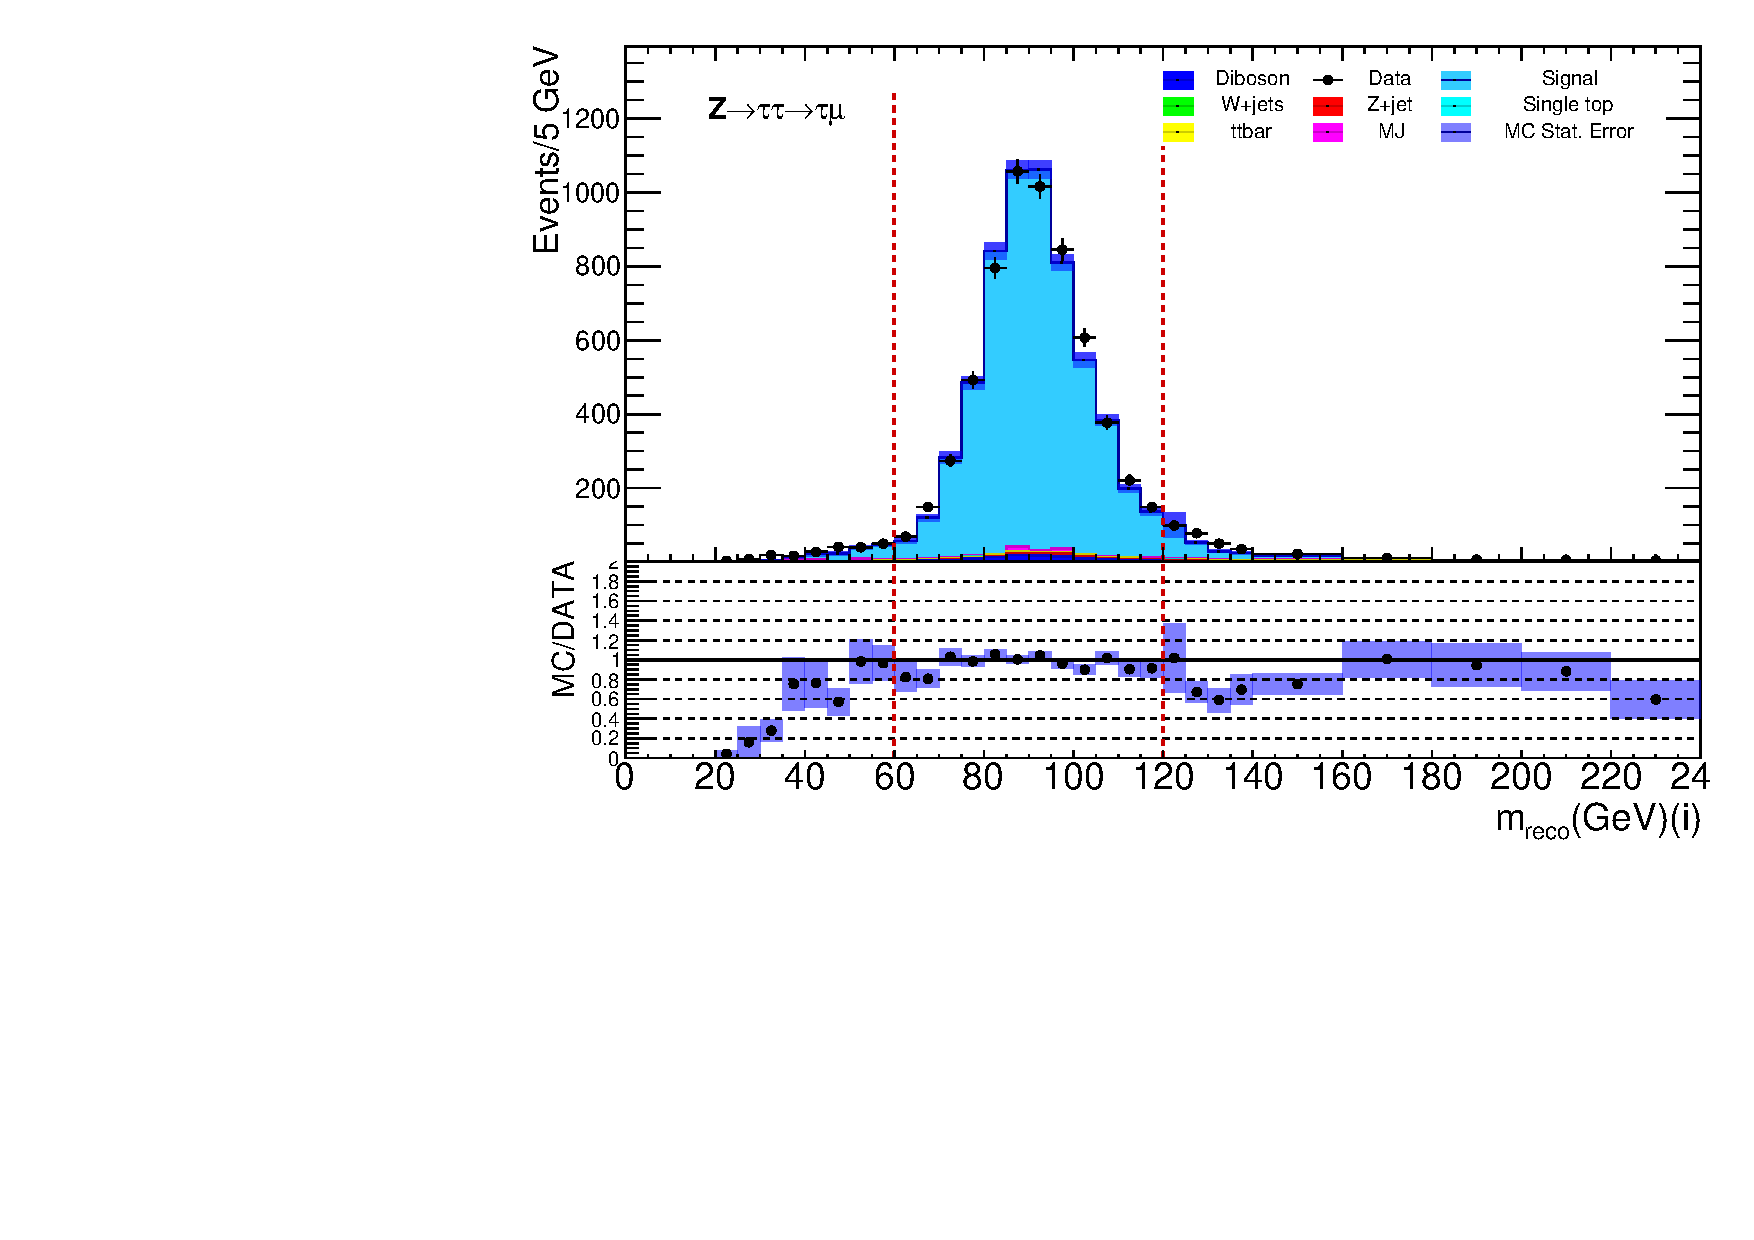
\includegraphics[width=0.50\textwidth]{figures/Fig4a}}}\hfill
	\subfloat[]{\label{Fig4b}{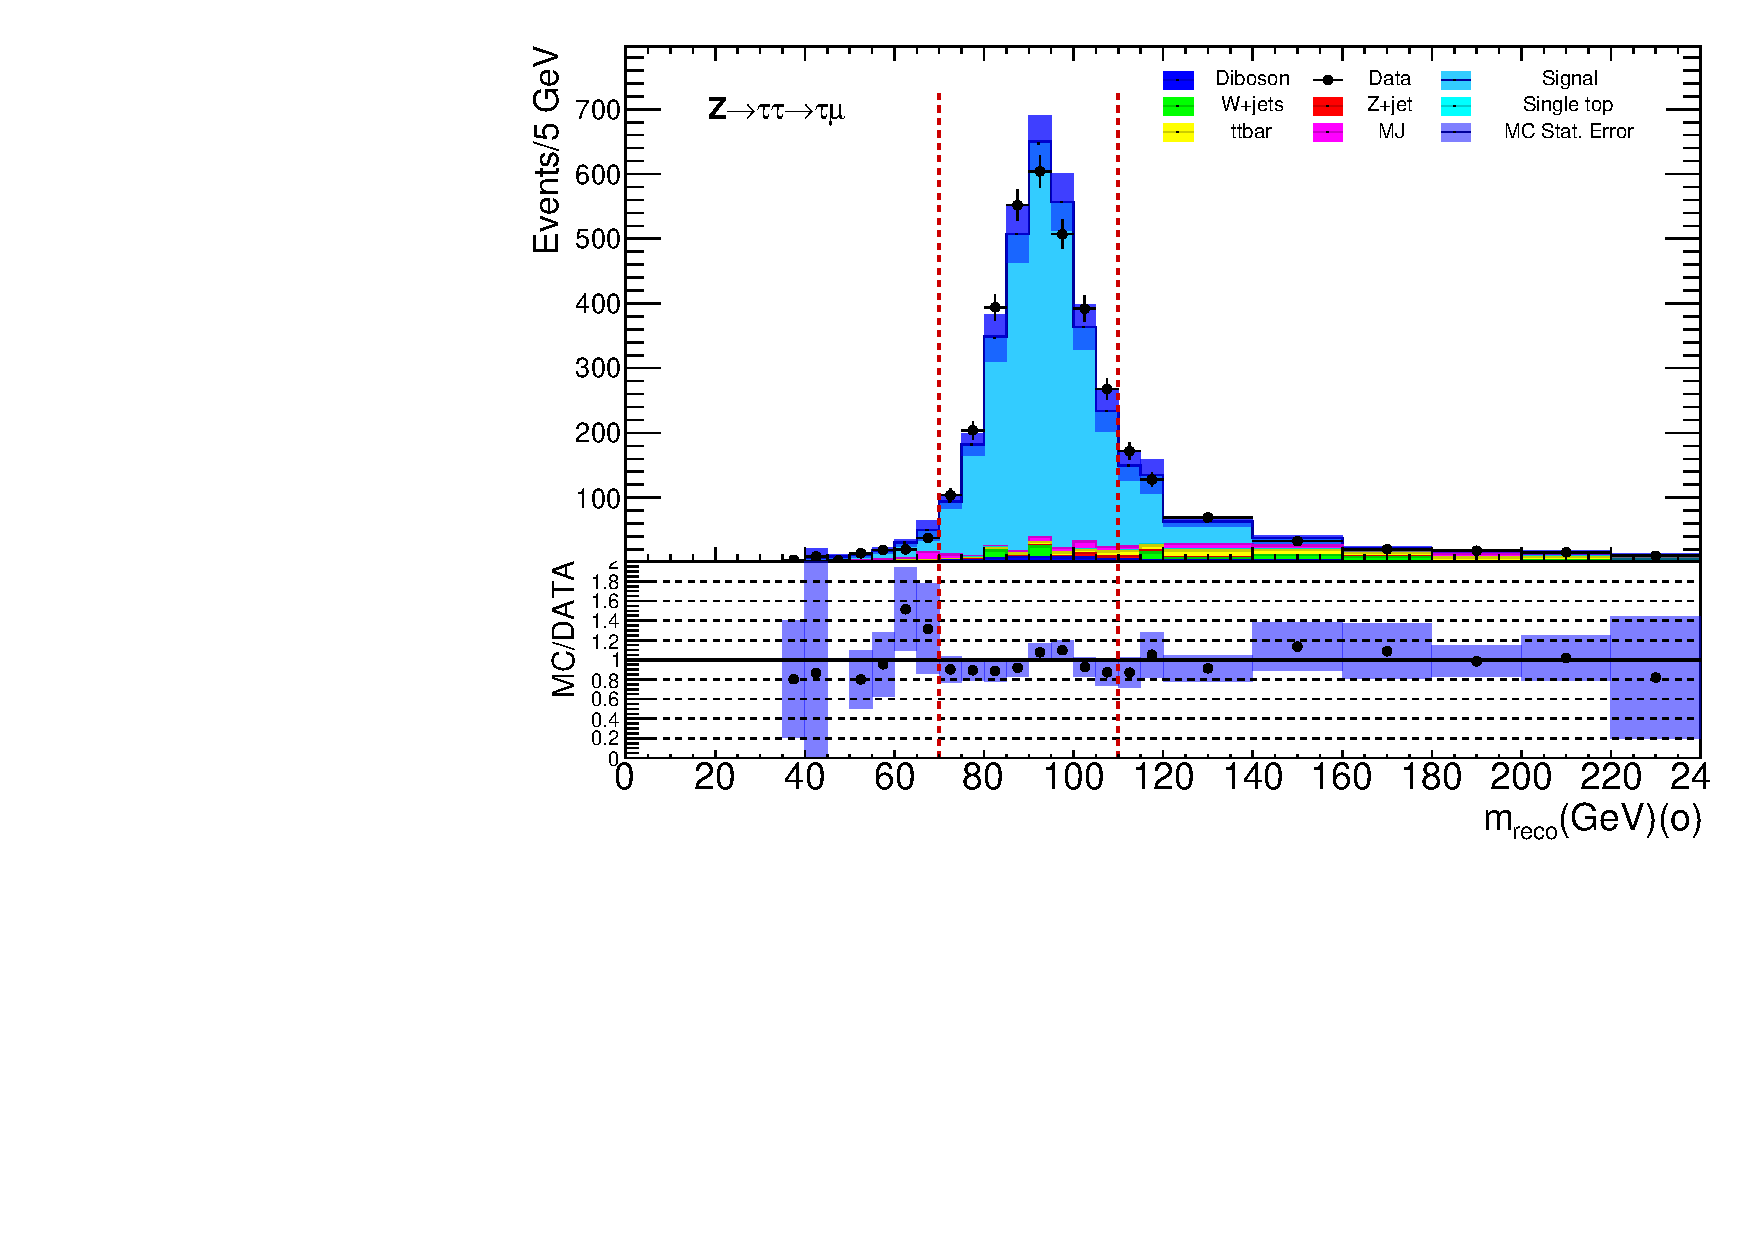
\includegraphics[width=0.50\textwidth]{figures/Fig4b}}}
	\caption{$\mreco$ distribution for the in-between region (a) and the outside region (b). All the other cuts have been applied apart from the one being plotted.}
	\label{Fig4}
\end{figure}

Furthermore, for the $Z\to\tauhad e$ final state, we add two cuts aimed to reject events where the $\tauhad$ candidate is faked by an electron. First, a requirement on the invariant mass of the electron and $\tauhad$ candidate is applied, $m(e,\tauhad)<80$ GeV. Then, we make use of an ID algorithm trained to discriminate electrons from real $\tauhad$. We require, eBDTScore$\geq 0.05$. The distributions for these variables are shown in Fig.\ref{Fig5}.
\begin{figure}[htbp]
	\centering
	\subfloat[]{\label{Fig5a}{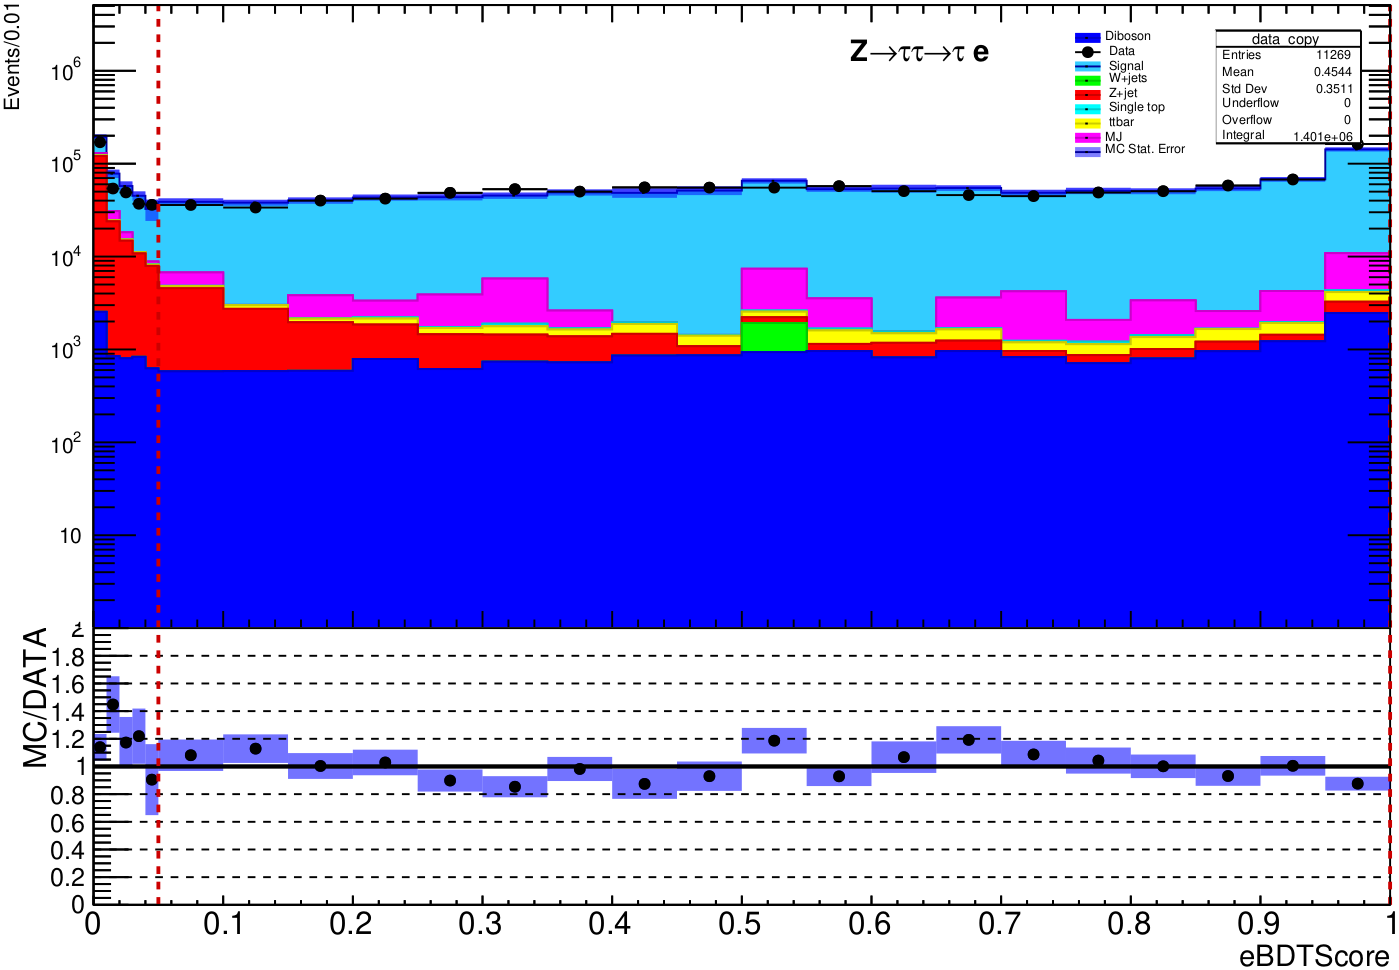
\includegraphics[width=0.50\textwidth]{figures/Fig5a}}}\hfill
	\subfloat[]{\label{Fig5b}{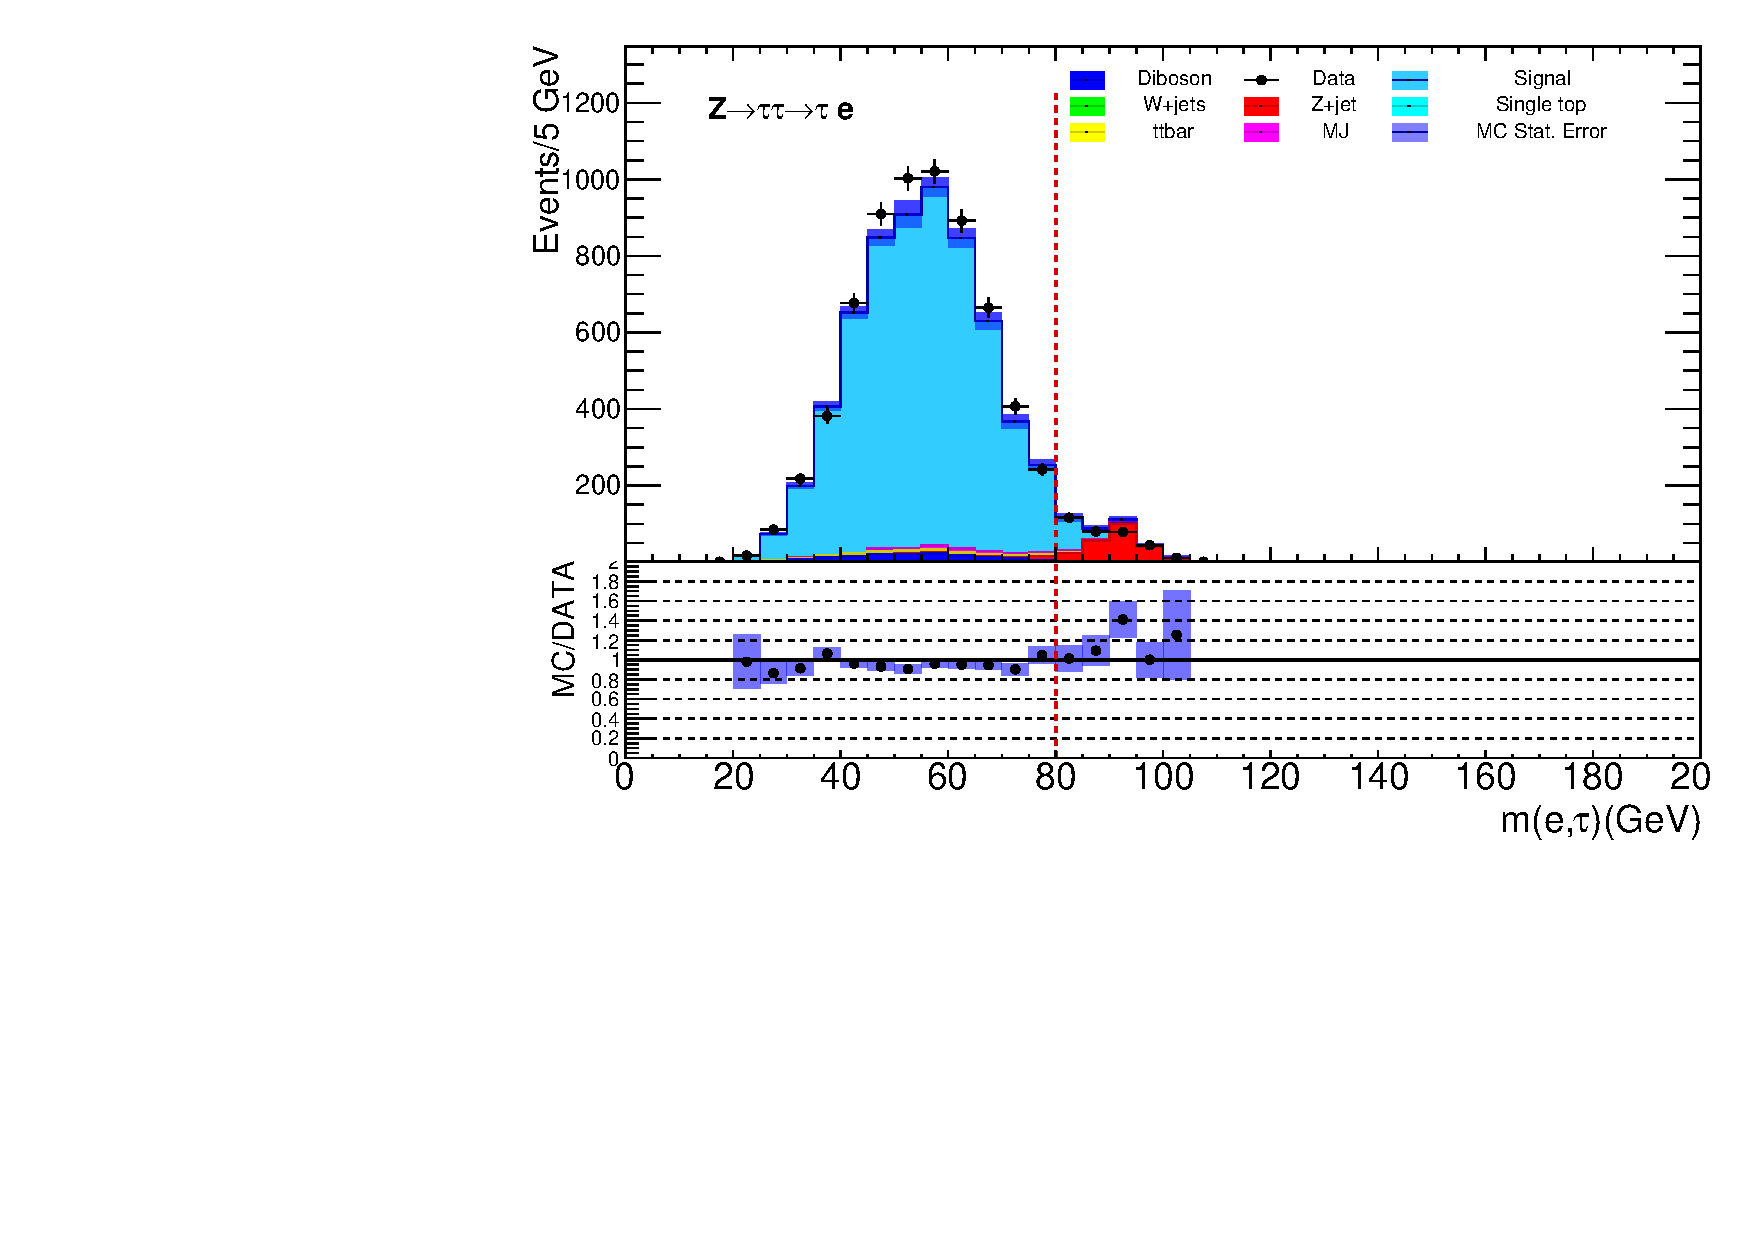
\includegraphics[width=0.50\textwidth]{figures/Fig5b}}}
	\caption{Distribution of the variables used to reject $\tauhad$ fakes coming from electrons. On the right $m(e,\tauhad)$ distribution (a) and on the left the eBDTScore distribution (b). All the other cuts have been applied apart from the one being plotted.}
	\label{Fig5}
\end{figure}

Finally, in order to measure the tau ID SFs in the high-$p_T$ region we select events where $p_T(\tauhad)\geq 45$ GeV. The $p_T$ distributions for $\tauhad$ candidates are shown in Fig.\ref{Fig6} for the in-between and outside regions. A side by side comparison of the $Z\to\tauhad\mu$ and $Z\to\tauhad e$ cut distributions can be found in A\ref{DistComparisons}.
\begin{figure}[htbp]
	\centering
	\subfloat[]{\label{Fig6a}{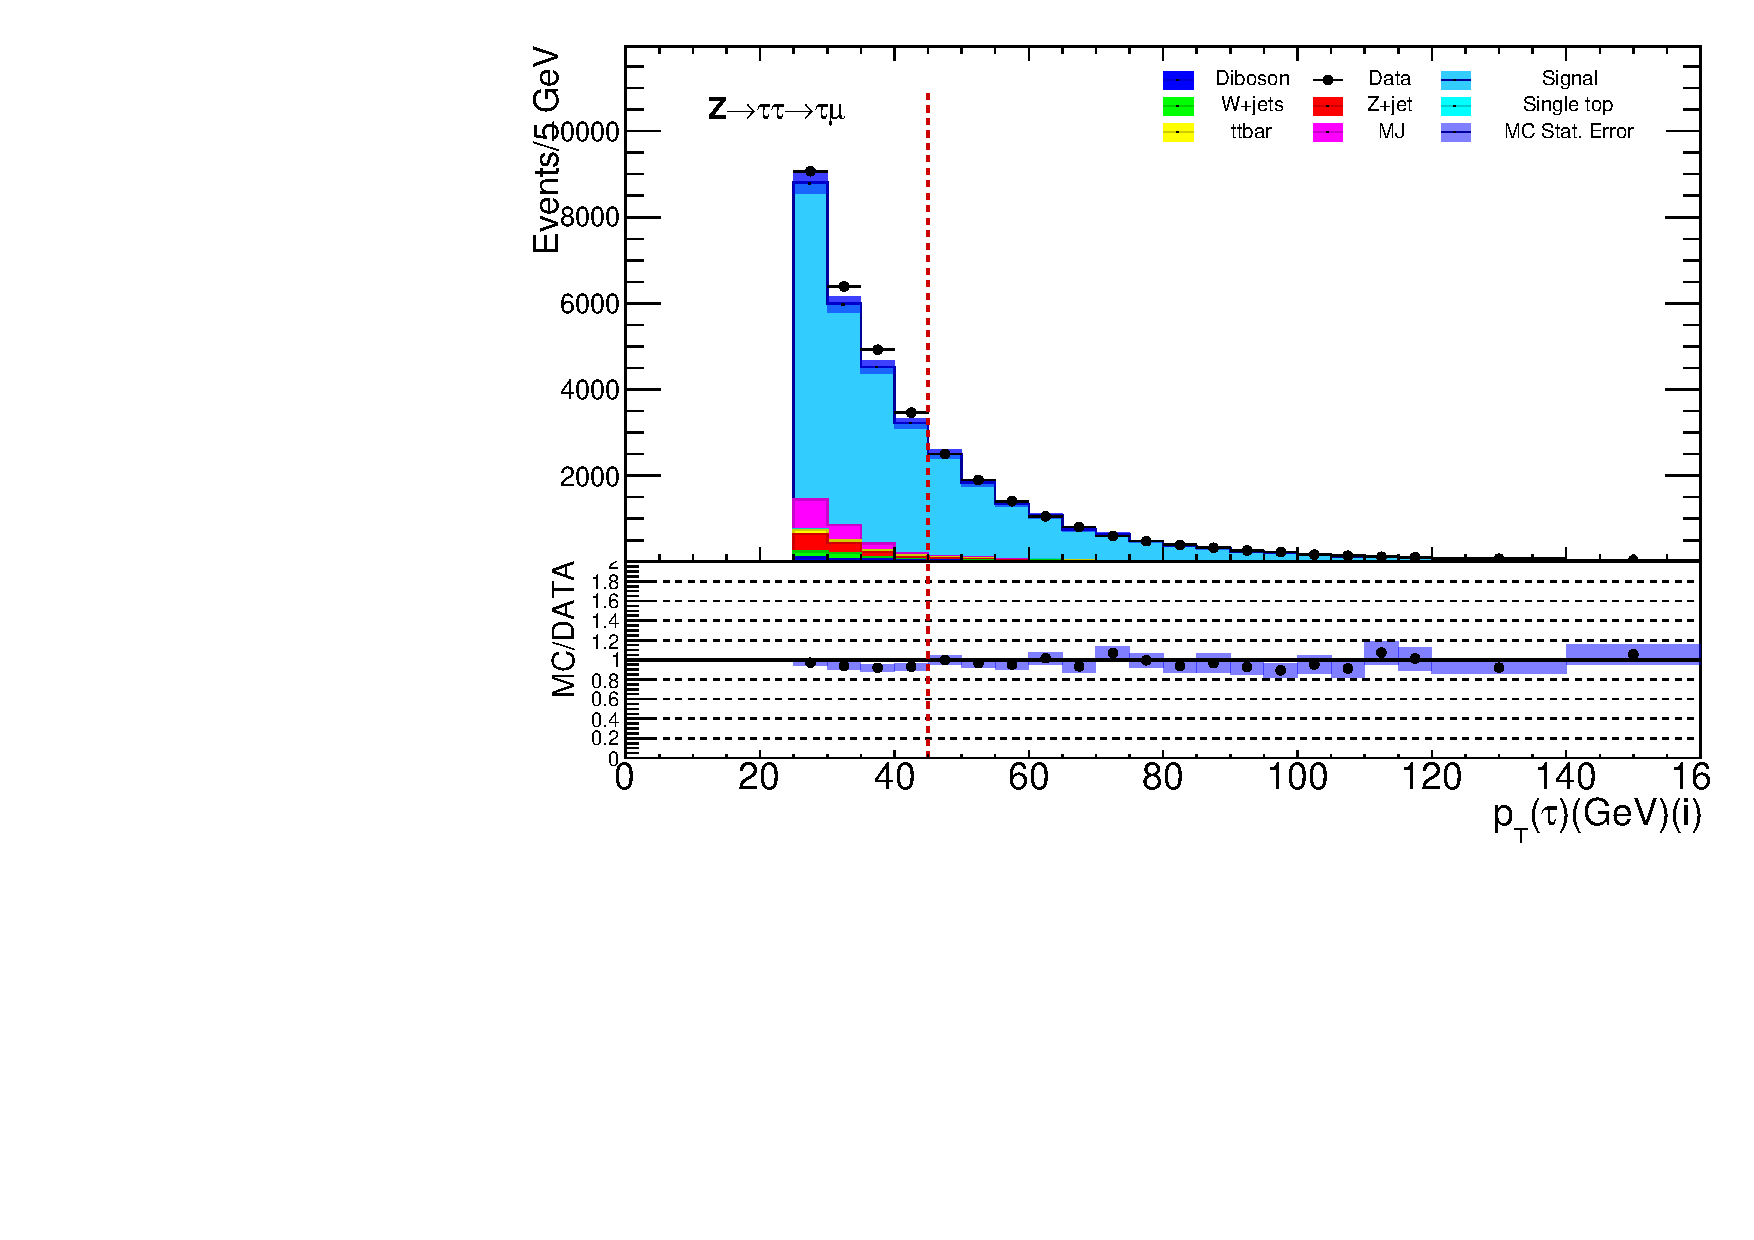
\includegraphics[width=0.50\textwidth]{figures/Fig6a}}}\hfill
	\subfloat[]{\label{Fig6b}{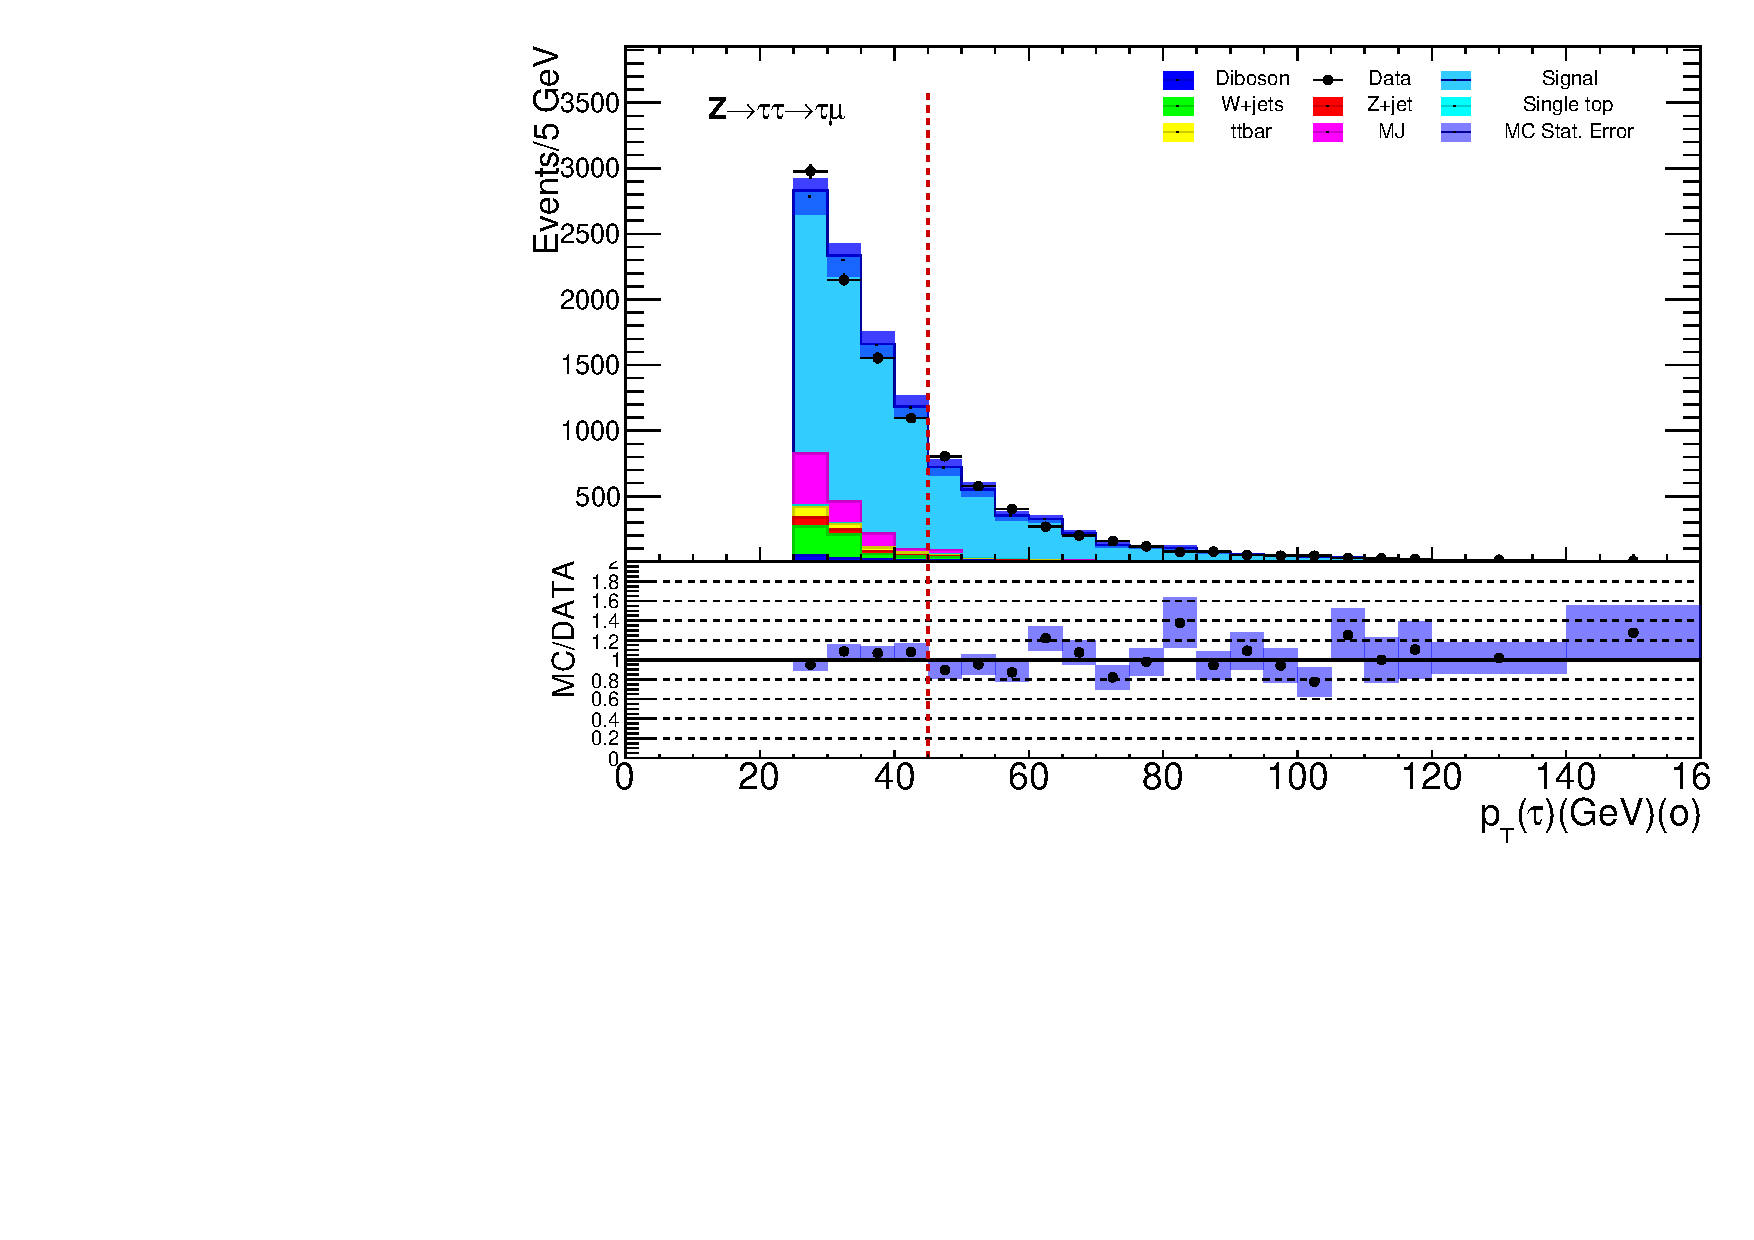
\includegraphics[width=0.50\textwidth]{figures/Fig6b}}}
	\caption{$p_T(\tauhad)$ distribution for the in-between (a) and outside (b) regions. All the other cuts have been applied apart from the one being plotted.}
	\label{Fig6}
\end{figure} 
\subsubsection{$\Zll$ Events}\label{sec3.3.2}
As described in Sec. \ref{sec3.2}, we will divide the simulation to data ratio in $Z\to\tauhad\taulep$ events by the same quantity in $\Zll$ events. In this final state, our basic selection includes events with exactly two same flavour and opposite charge light-leptons. The same lepton triggers are used for this final state.

Events containing b-jets are vetoed in order to reject $t\bar{t}$ background. In addition, the same isolation and identification criterion is required to be passed by the leptons. A cut in the invariant mass of the light lepton pair is applied, $70<m(l_1,l_2)<110$ GeV. The corresponding distribution is shown in Fig. \ref{Fig7s}.

\begin{figure}[htbp]
	\centering
	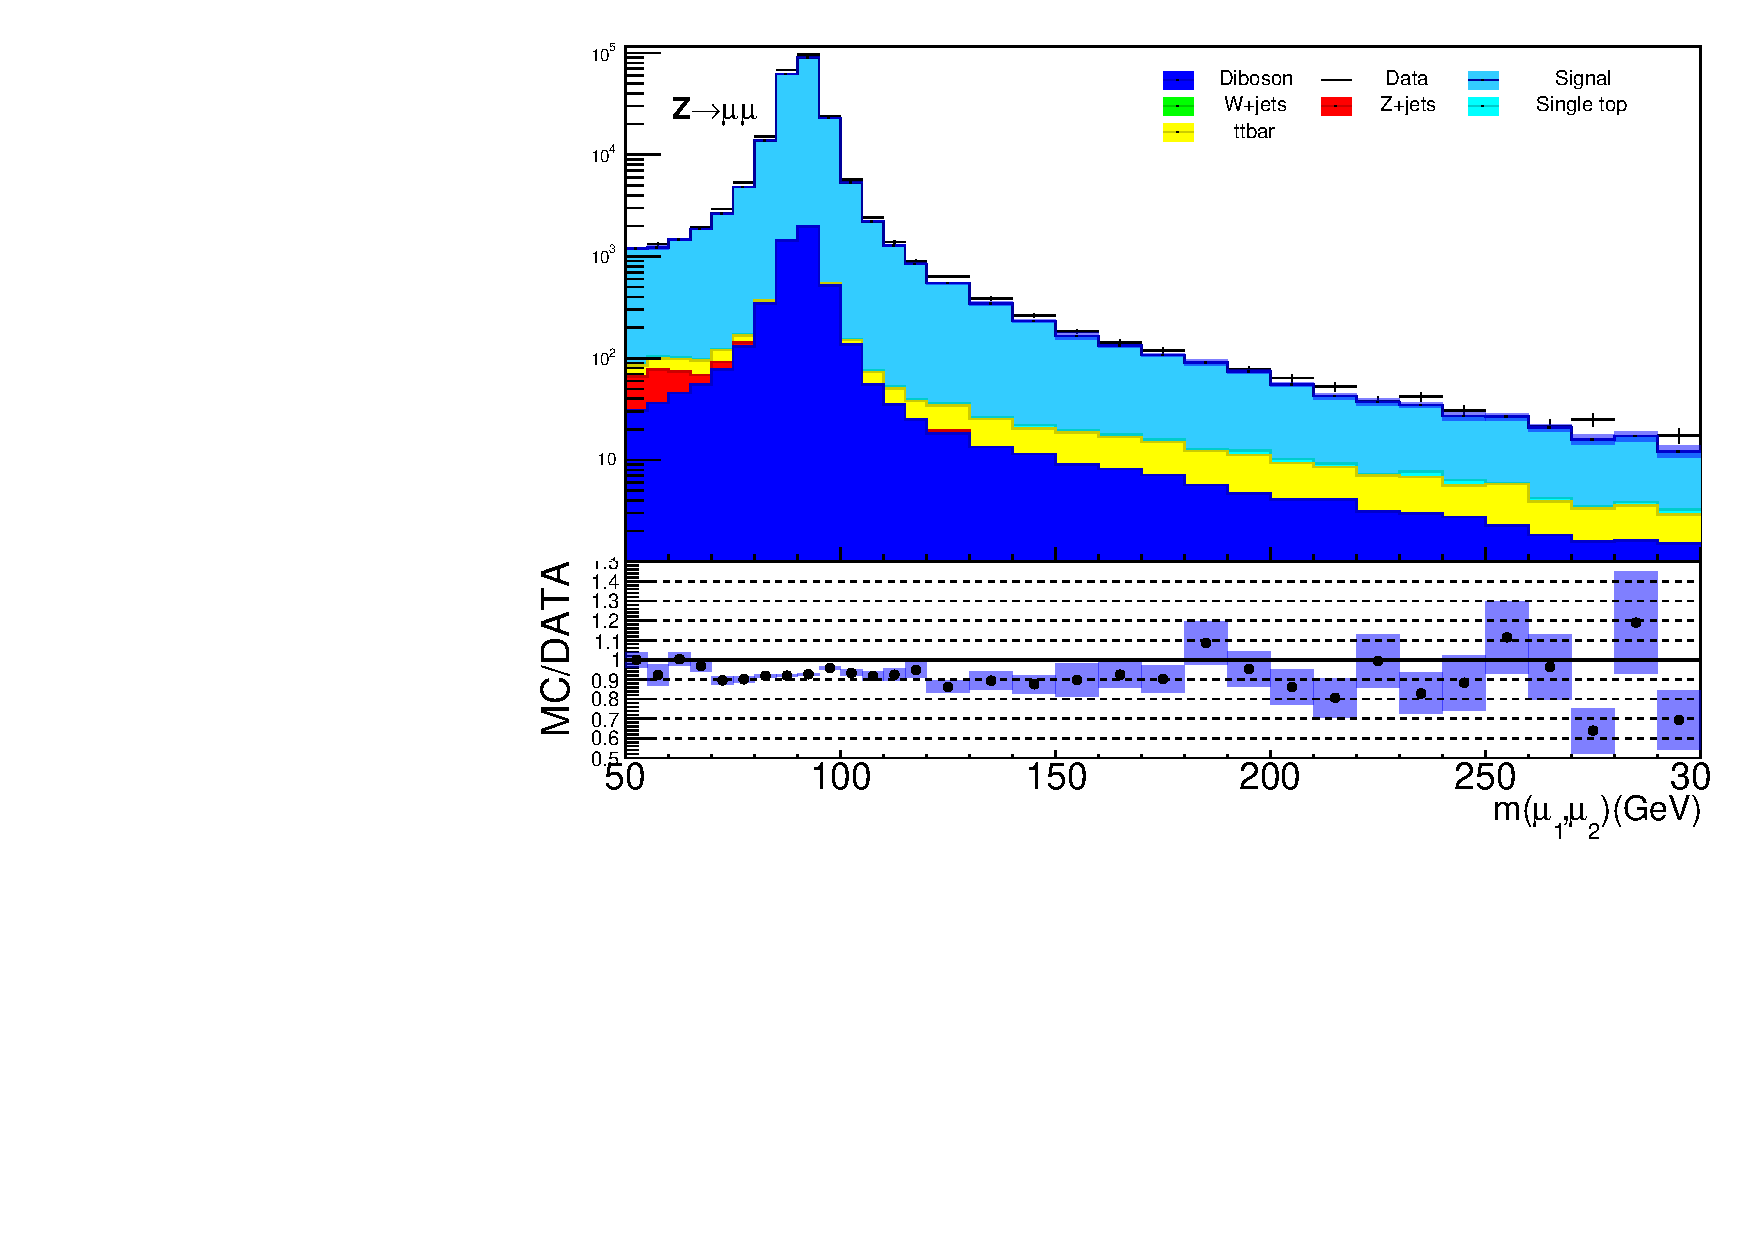
\includegraphics[width=0.6\textwidth]{figures/Fig7.pdf}
	\caption{$m(l_1,l_2)$ distribution for the $Z\to\mu\mu$ final state. All the other cuts have been applied apart from the one being plotted. In this and all subsequent figures, the ATLAS data is shown as points with error bars, corresponding to the statistical uncertainties. The detector-level predictions are shown as the coloured histograms, with the colour code as given in the plots. The region included in the final sample is $70<m(l_1,l_2)<11	0$ GeV. The lower section of each plot shows the ratio of prediction to real data. The uncertainties on the predictions represent the MC statistical uncertainties. These uncertainties are shown as the blue shaded region.}
	\label{Fig7s}
\end{figure}

Since the visible products of the tau decay only carry a part of the original tau $\pt$, we need to cut harder on the light leptons produced in $\Zll$ events. Therefore, to approximately match the kinematic phase space between  $Z\to\tauhad\taulep$ and $\Zll$ events many different values for the $\Delta\phi (l_1,l_2)$ and the $\pt$ of the leptons have been explored. For the angular separation, the best match is to require $\Delta\phi (l_1,l_2)\leq 1.0$ rad, the $\Delta\phi (l_1,l_2)$ distribution is shown in Fig. \ref{Fig8s}. Regarding the transverse momentum of the leptons, an initial offline requirement of $\pt(l_1)\geq 50$ and $\pt(l_2)\geq 47$ GeV is applied. To be able to match the high-$\pt$ $\tauhad$ candidates a further cut of 30 GeV is randomly applied in one of the leptons. This last part is due to the fact that the light-leptons are ordered in $\pt$ and not always the hardest tau is the $\tauhad$ candidate. The resulting distributions are shown in Fig. \ref{Fig9}.
\begin{figure}[htbp]	
	\centering
	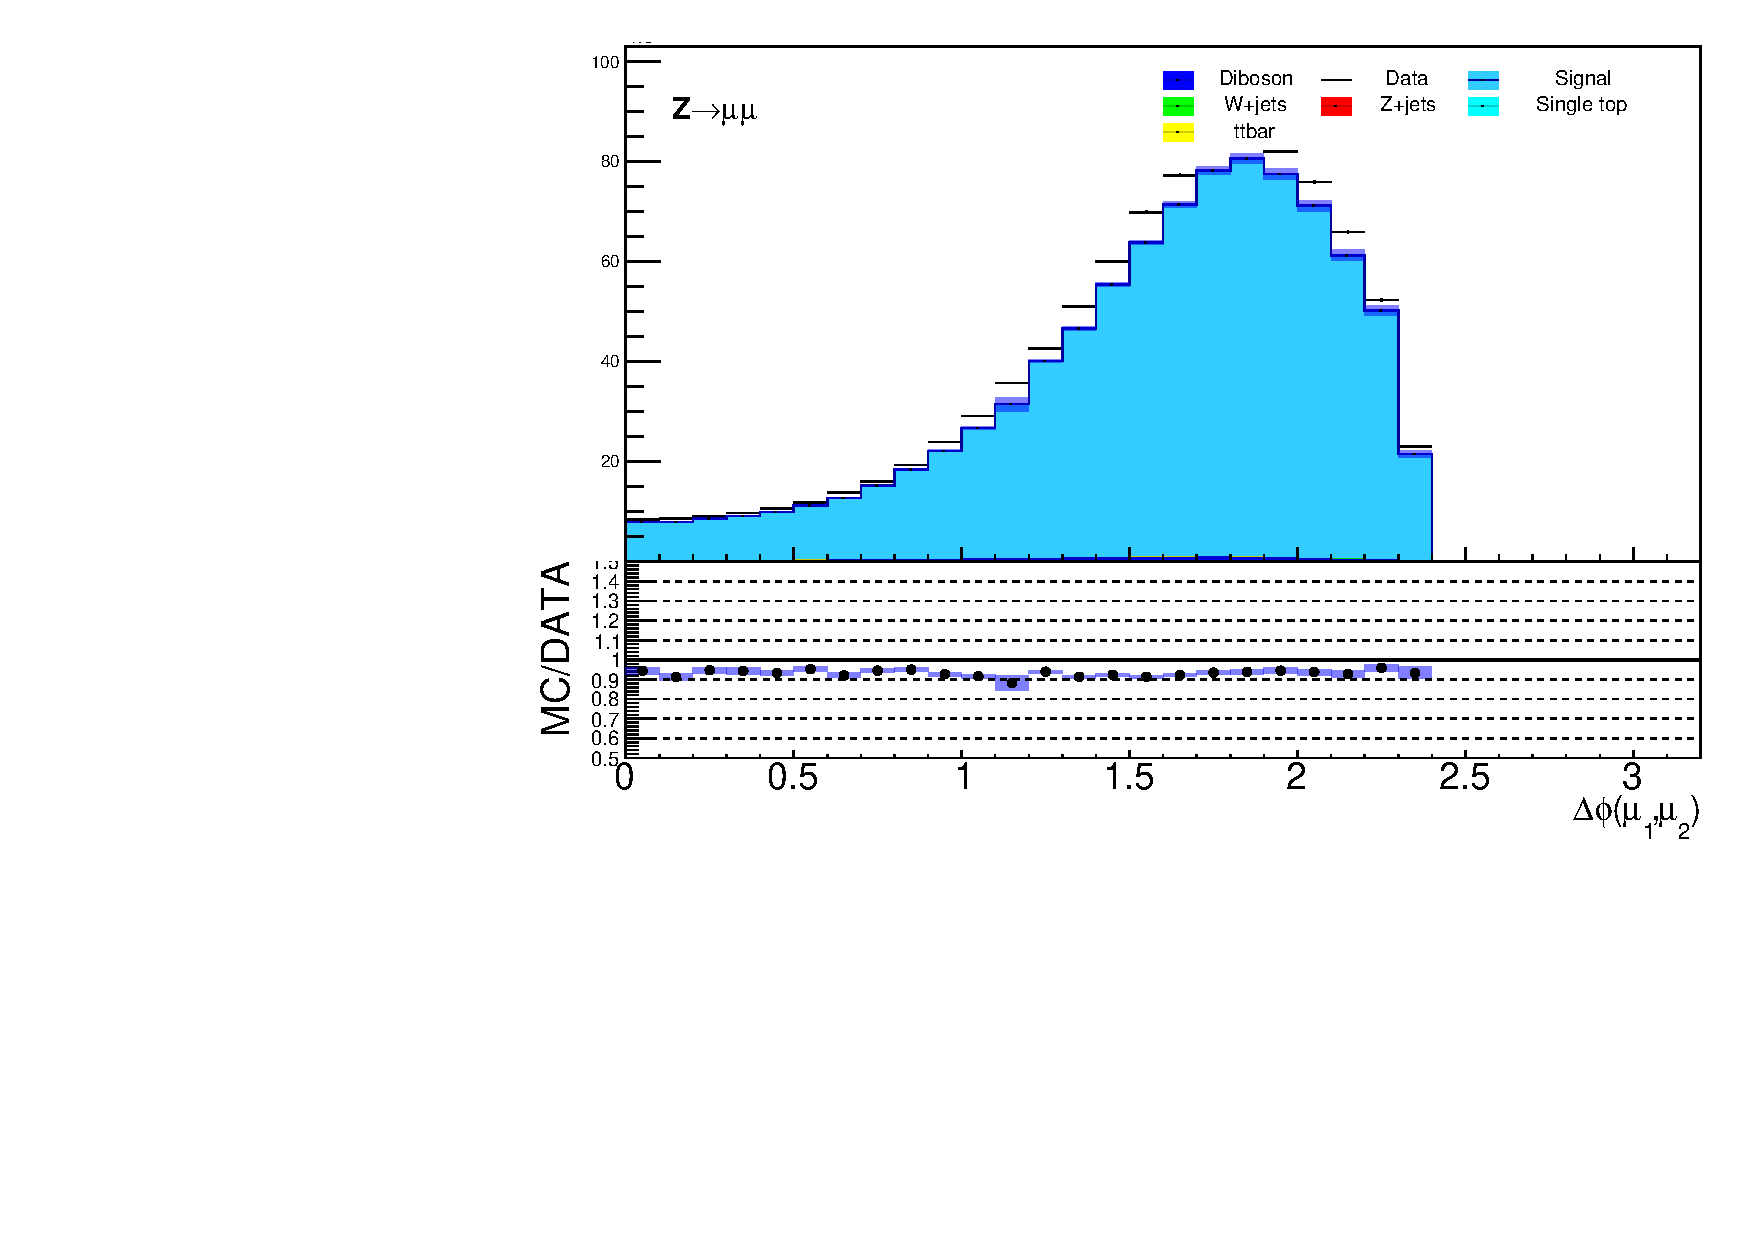
\includegraphics[width=0.6\textwidth]{figures/Fig8.pdf}
	\caption{Distribution of $\Delta\phi (l_1,l_2)$ for the $Z\to\mu\mu$ final state. The region included in the final selection is $\Delta\phi (l_1,l_2)\leq 1.0$ rad.}
	\label{Fig8s}
\end{figure}
\begin{figure}[htbp]
	\centering
	\subfloat[]{\label{Fig9a}{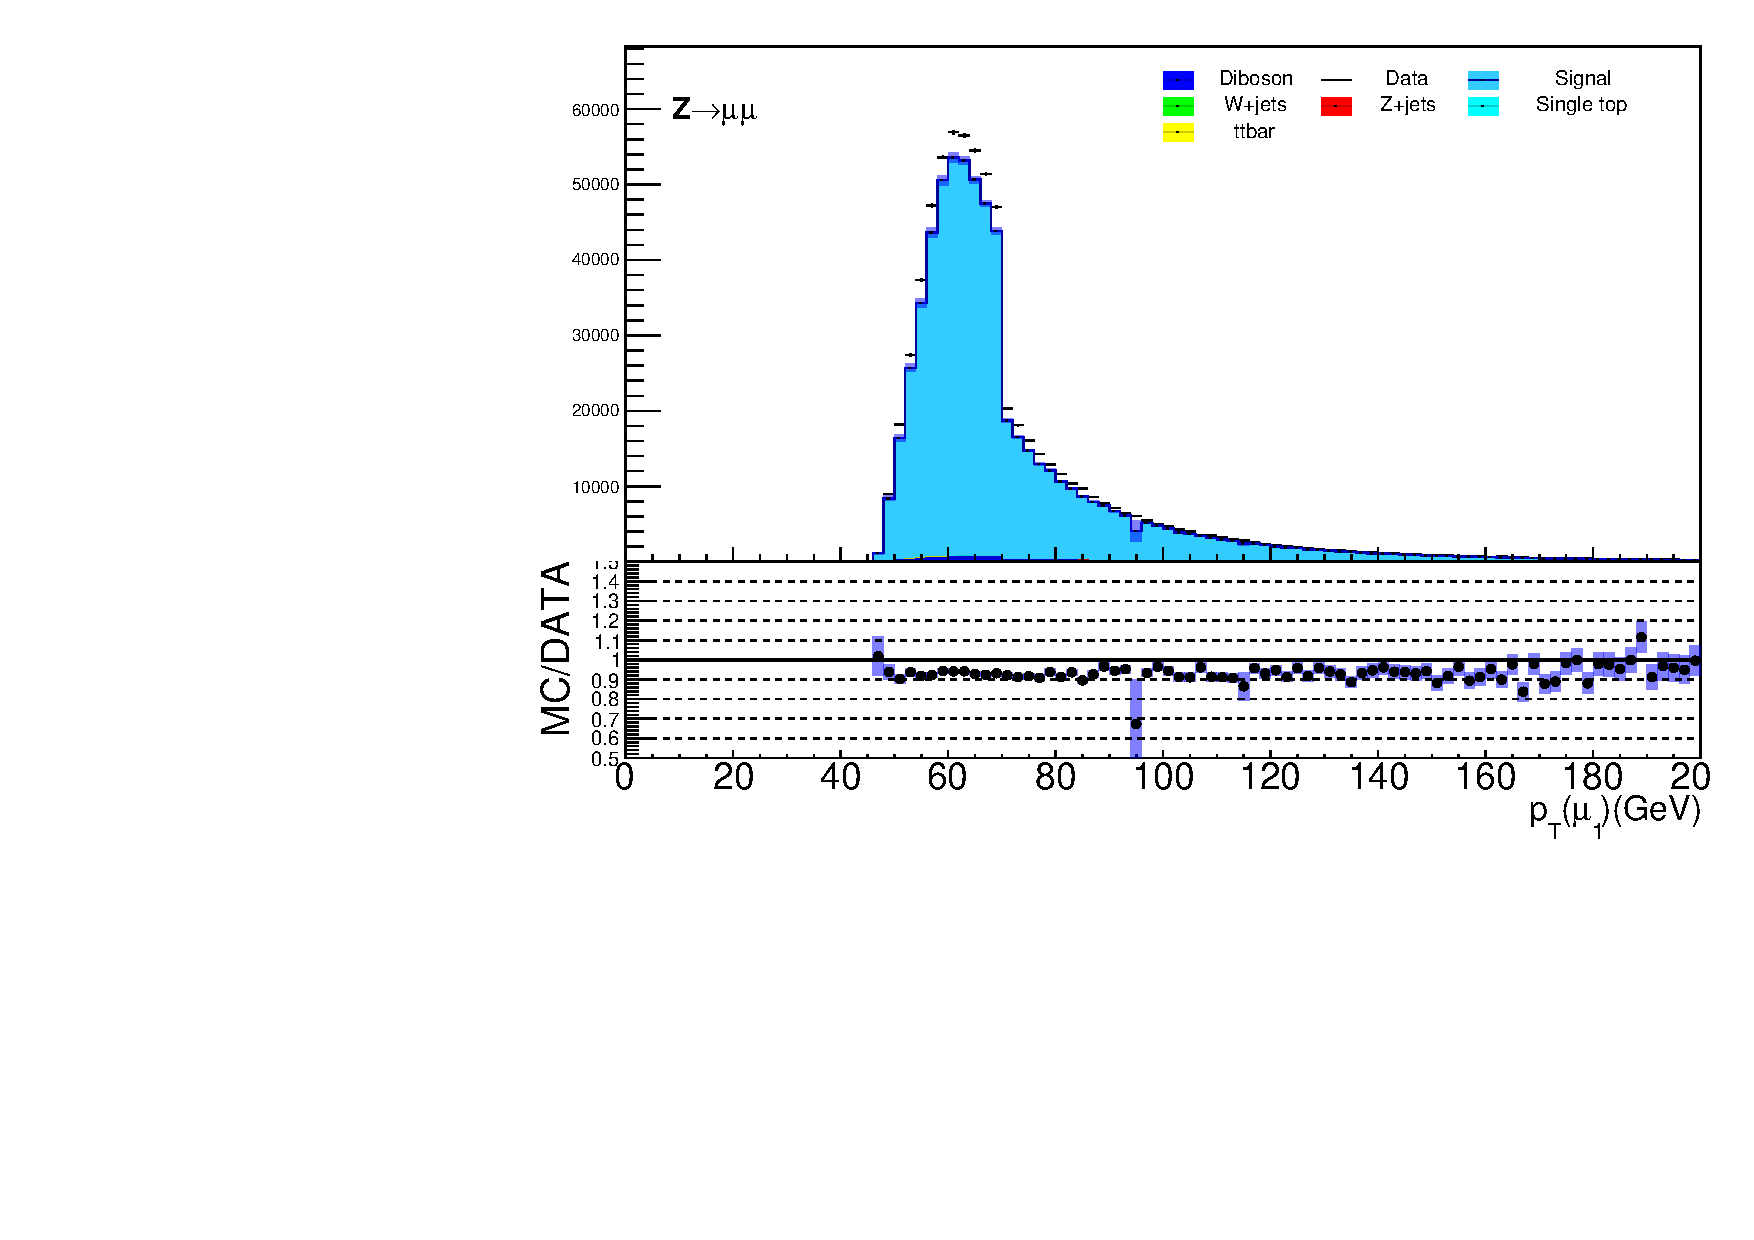
\includegraphics[width=0.50\textwidth]{figures/Fig9a}}}\hfill
	\subfloat[]{\label{Fig9b}{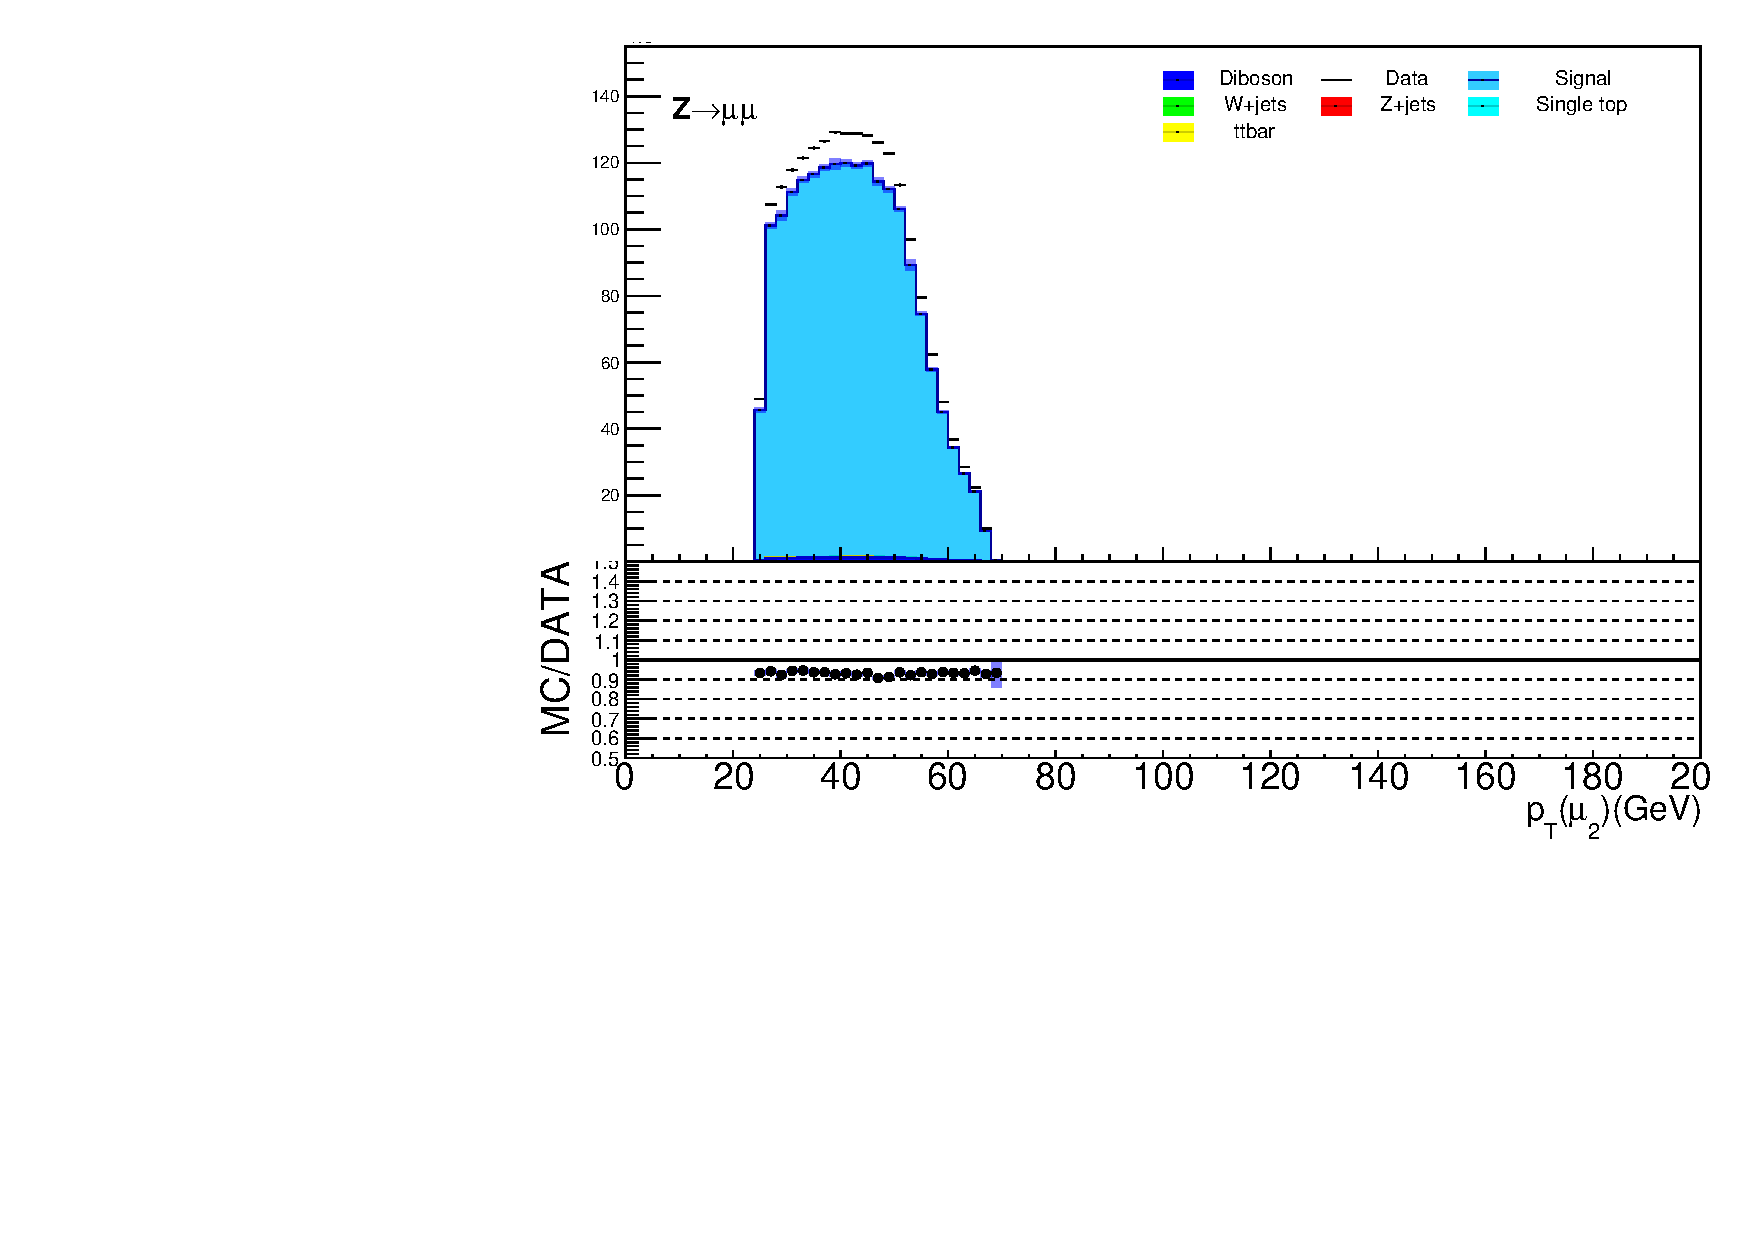
\includegraphics[width=0.50\textwidth]{figures/Fig9b}}}
	\caption{$\pt$ distributions for $Z\to\mu\mu$ events.}
	\label{Fig9}
\end{figure}

The reconstructed and truth Z$(\pt)$ distributions with the best match cuts between $\Zll$ and $Z\to\tauhad\taulep$ events are shown in Fig.\ref{Fig13} . A set of alternative selections, defined by varying the last lepton $\pT$ cut by 10 GeV have been studied. This aims to asses the effect of having different degree of kinematic match between $\Zll$ and $Z\to\tauhad\taulep$ final states. The corresponding truth Z$(\pt)$ distributions for every selection are shown in Fig.\ref{Fig14} .

\begin{figure}[htbp]
	\centering
	\subfloat[]{\label{Fig13a}{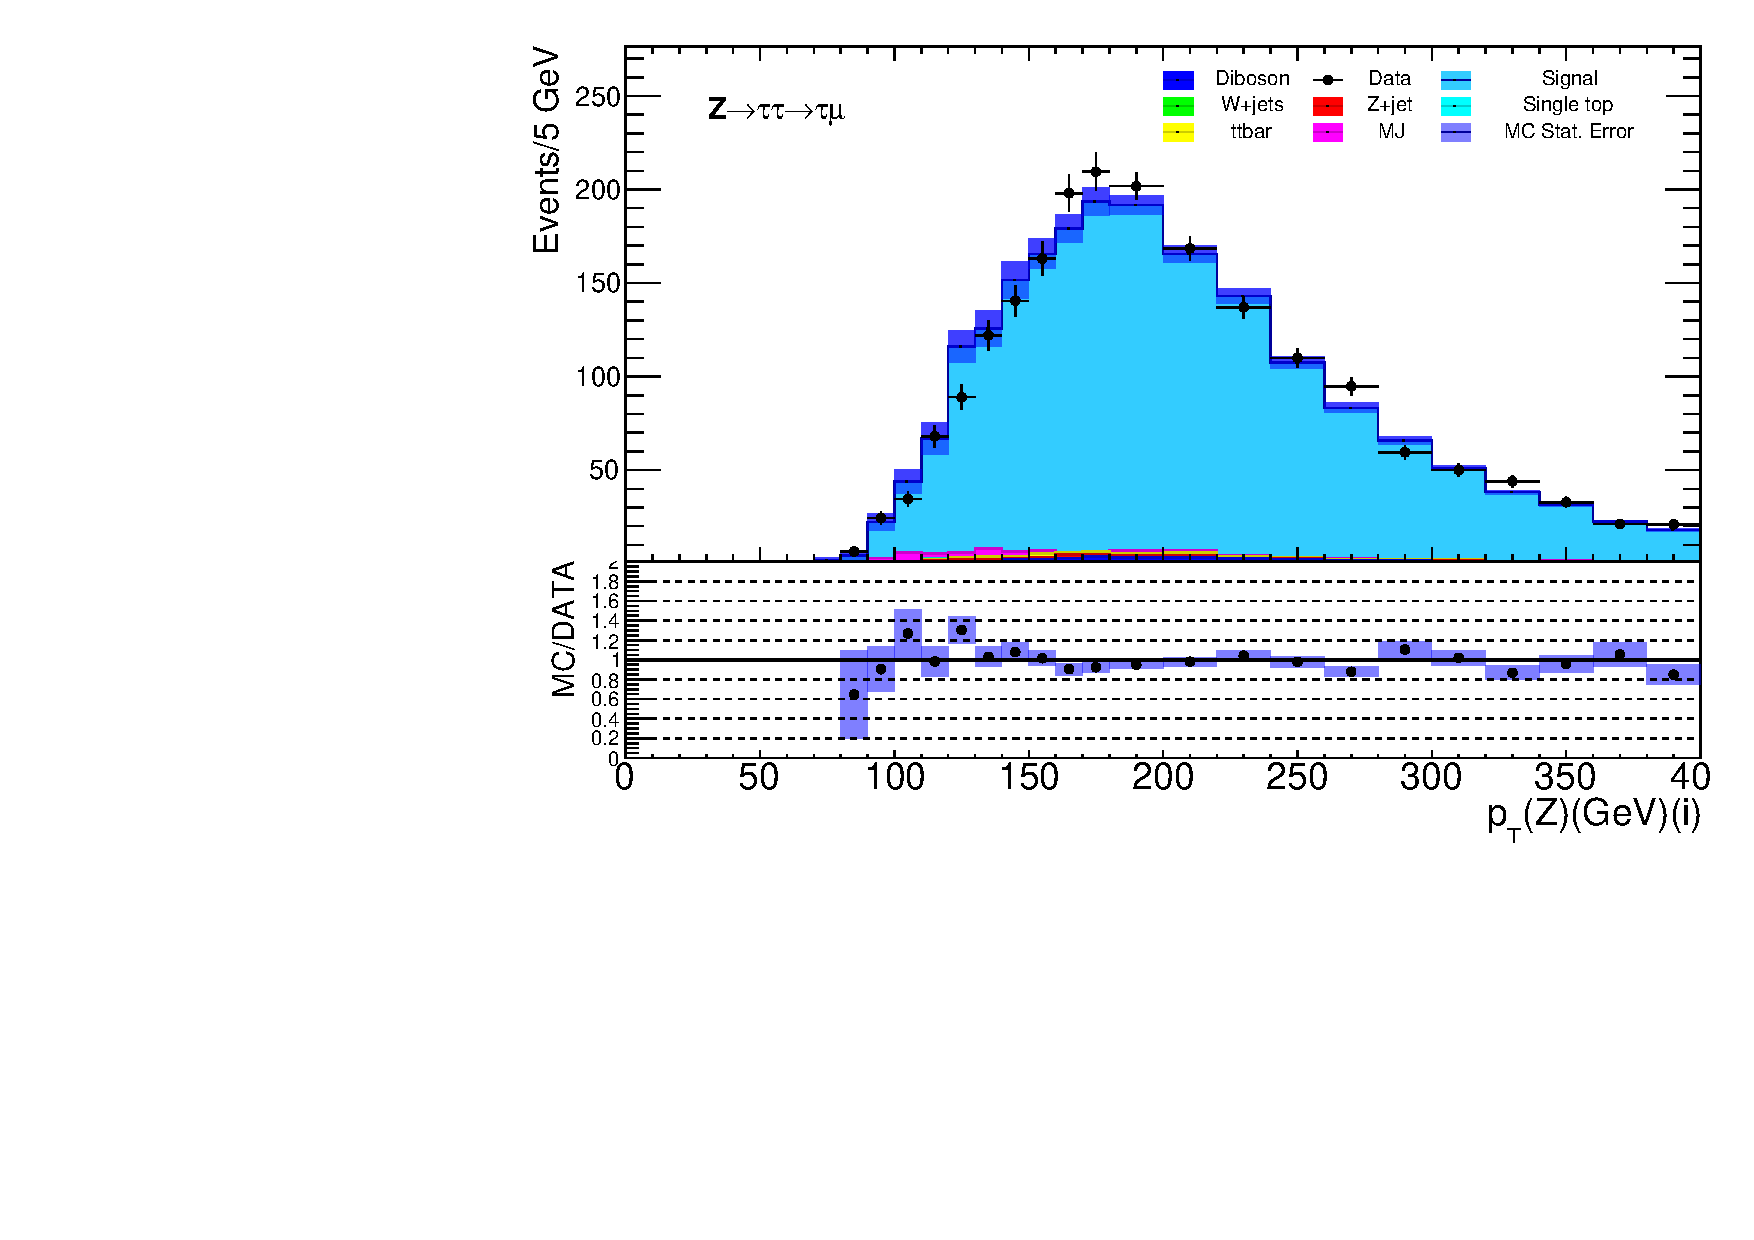
\includegraphics[width=0.50\textwidth]{figures/Fig13a.pdf}}}
	\subfloat[]{\label{Fig13b}{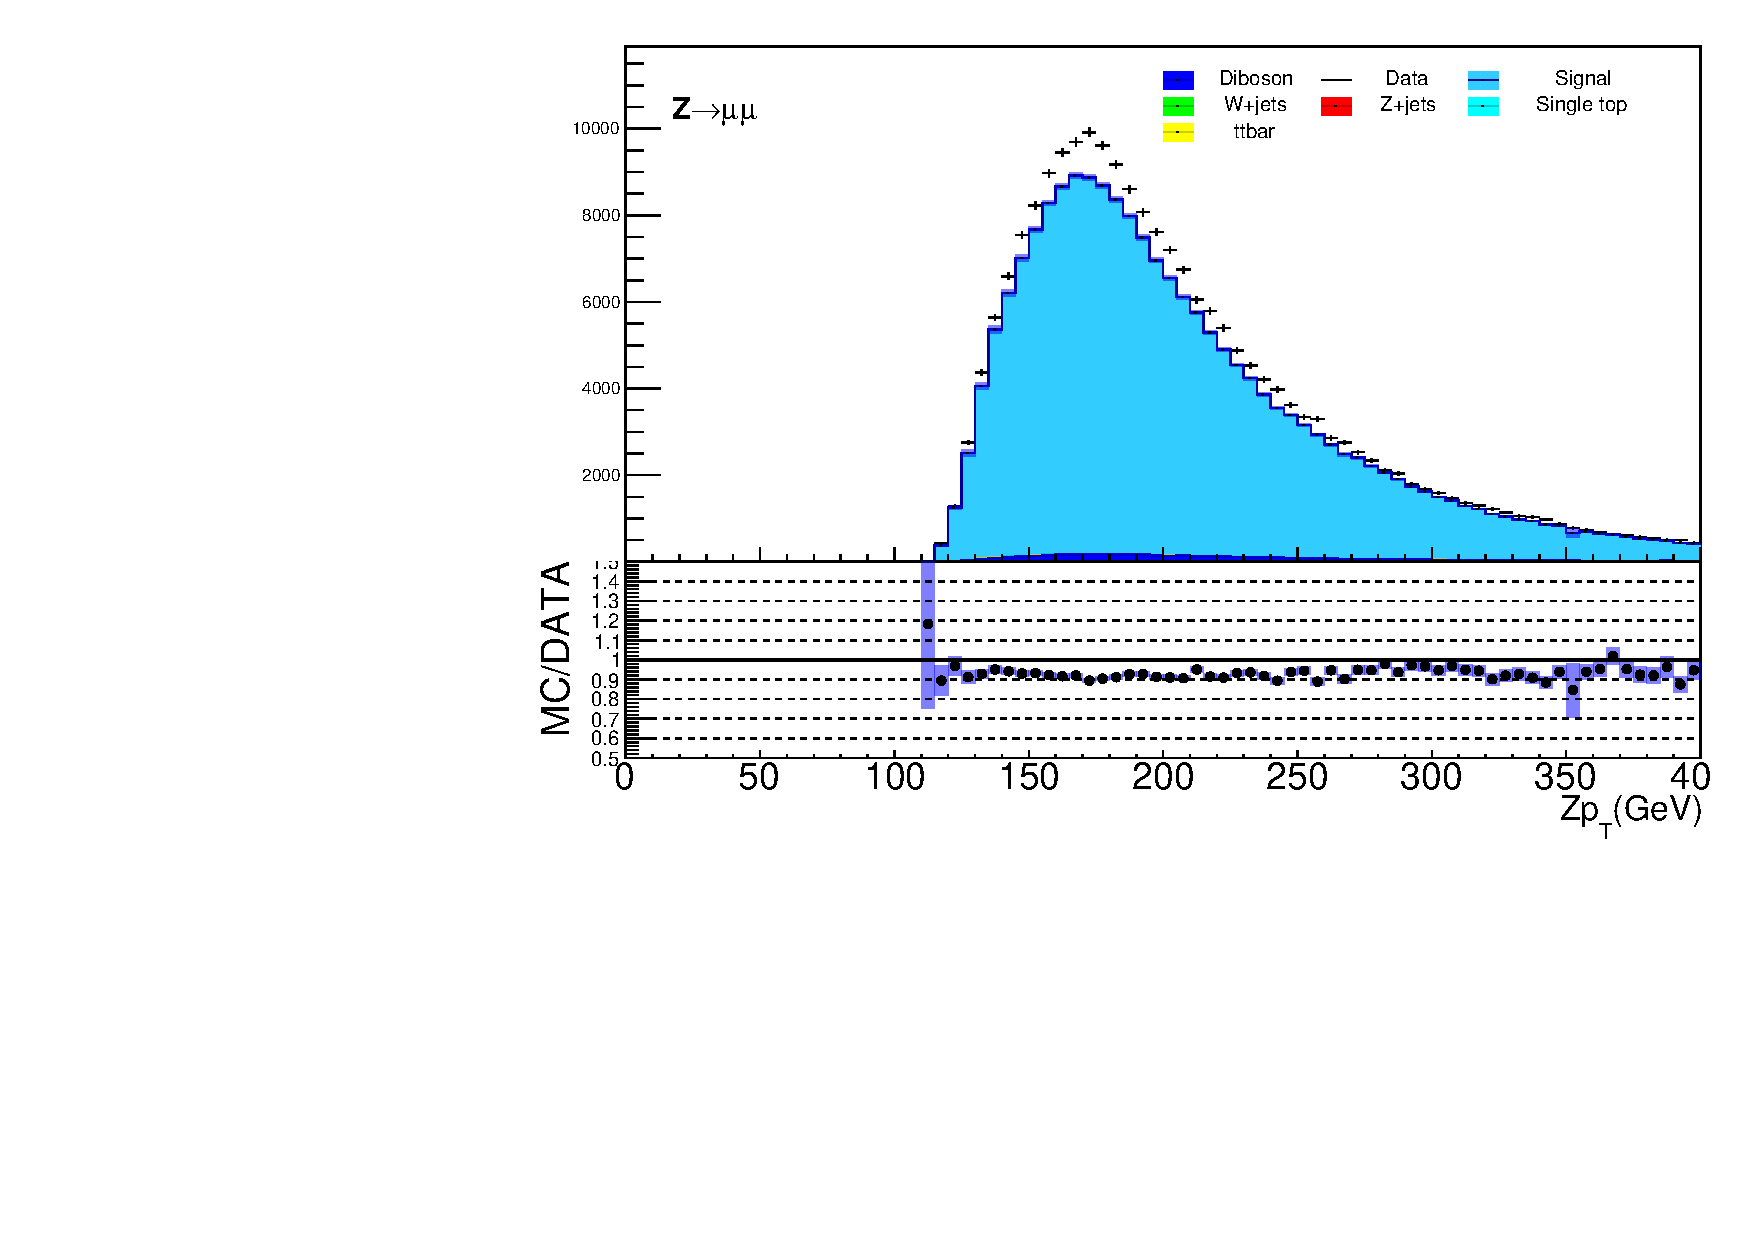
\includegraphics[width=0.50\textwidth]{figures/Fig13b.pdf}}}\hfill
	\subfloat[]{\label{Fig13c}{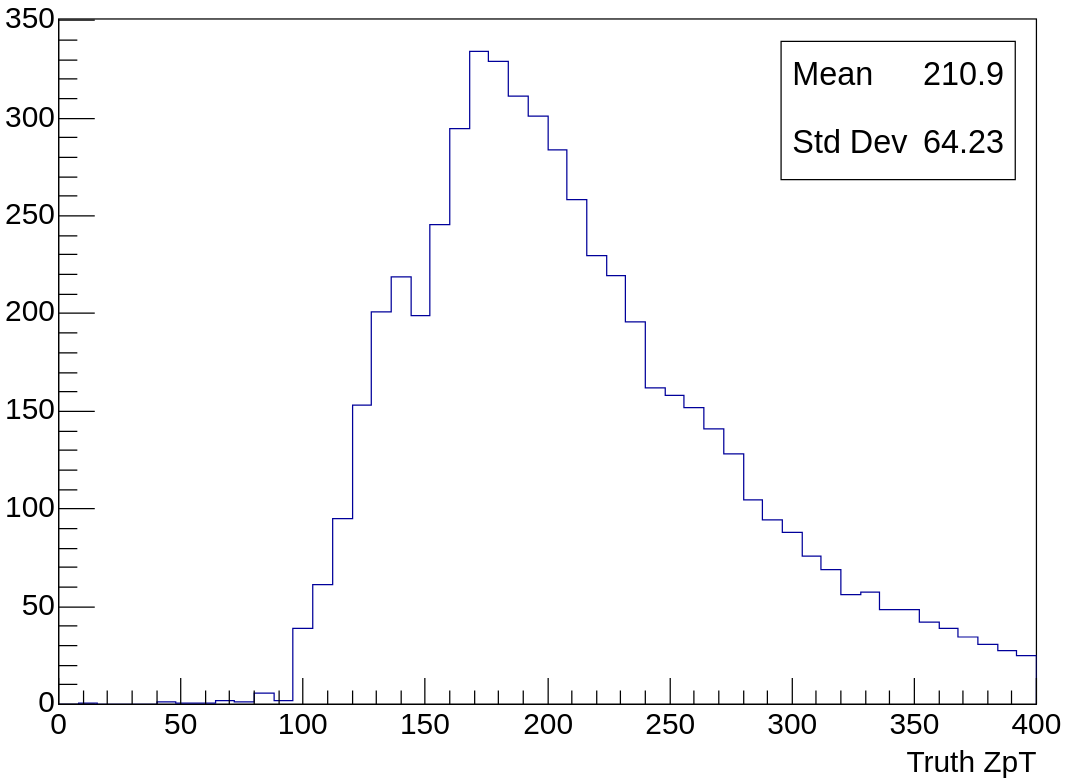
\includegraphics[width=0.50\textwidth]{figures/Fig13c.png}}}
	\subfloat[]{\label{Fig13d}{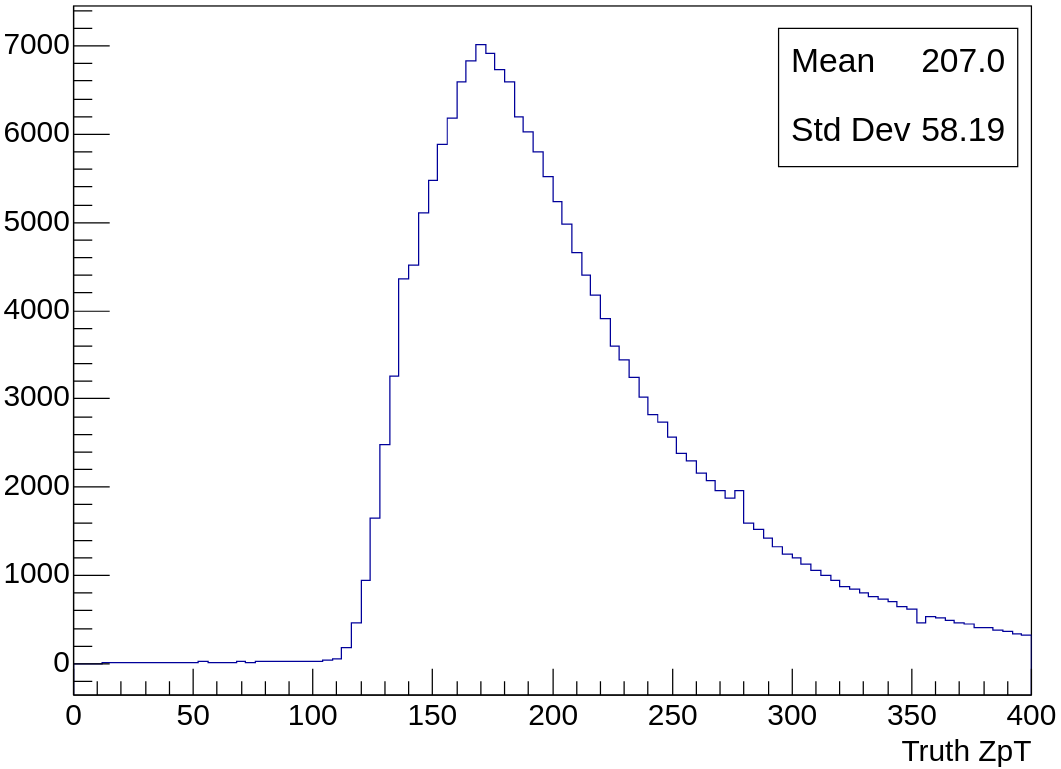
\includegraphics[width=0.50\textwidth]{figures/Fig13d.png}}}
	\caption{Left column represents the detector level (a) and truth level (c) Z$(\pt)$ distributions for $Z\to\tauhad\mu$ events. In the right column, the same variables are shown for the $Z\to\mu\mu$ final state.}
	\label{Fig13}
\end{figure}

\begin{figure}[htbp]
	\centering
	\subfloat[]{\label{Fig14a}{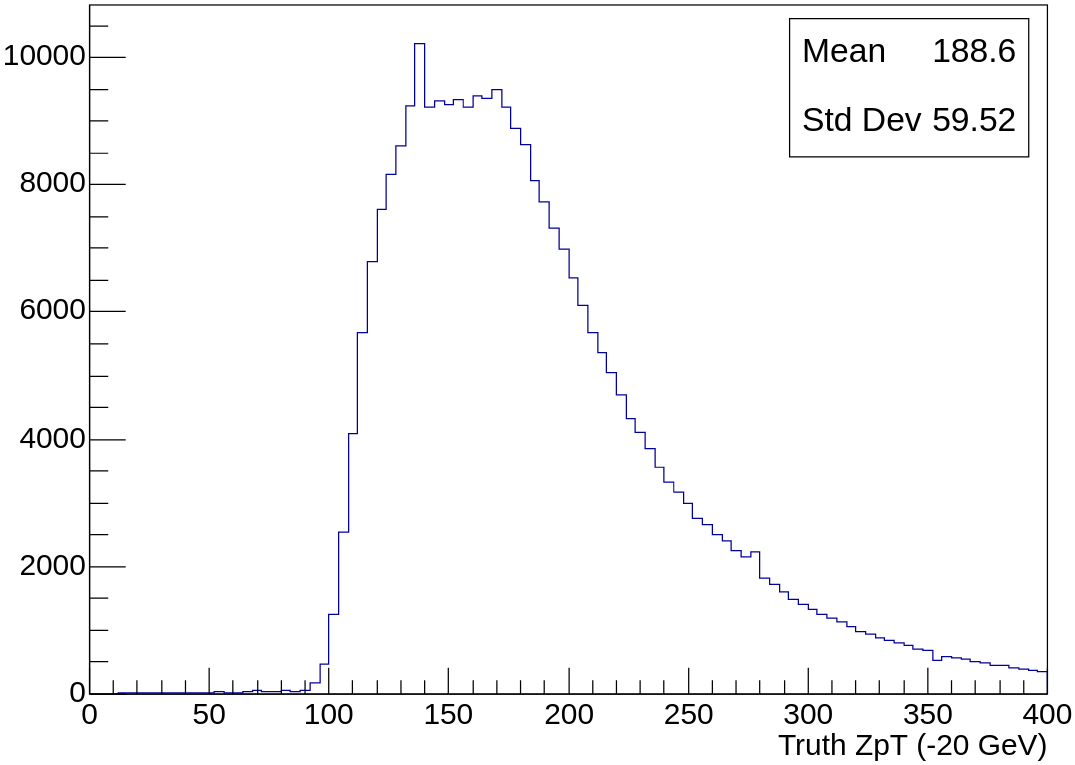
\includegraphics[width=0.50\textwidth]{figures/Fig14a.png}}}
	\subfloat[]{\label{Fig14b}{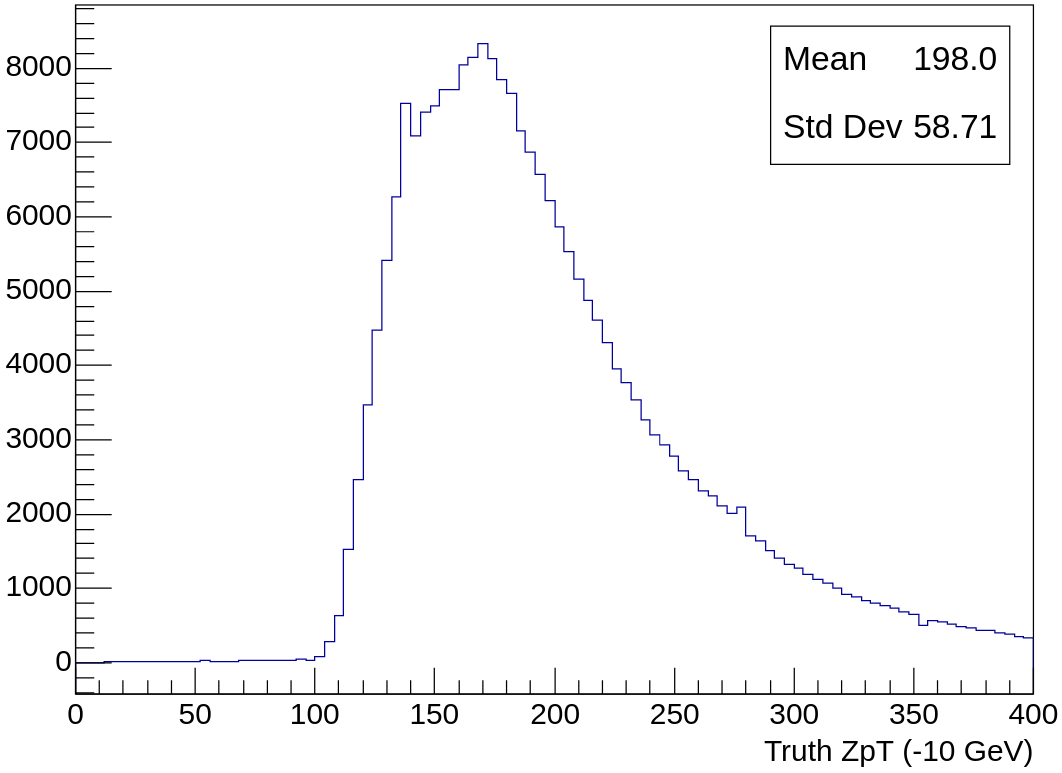
\includegraphics[width=0.50\textwidth]{figures/Fig14b.png}}}\hfill
	\subfloat[]{\label{Fig14c}{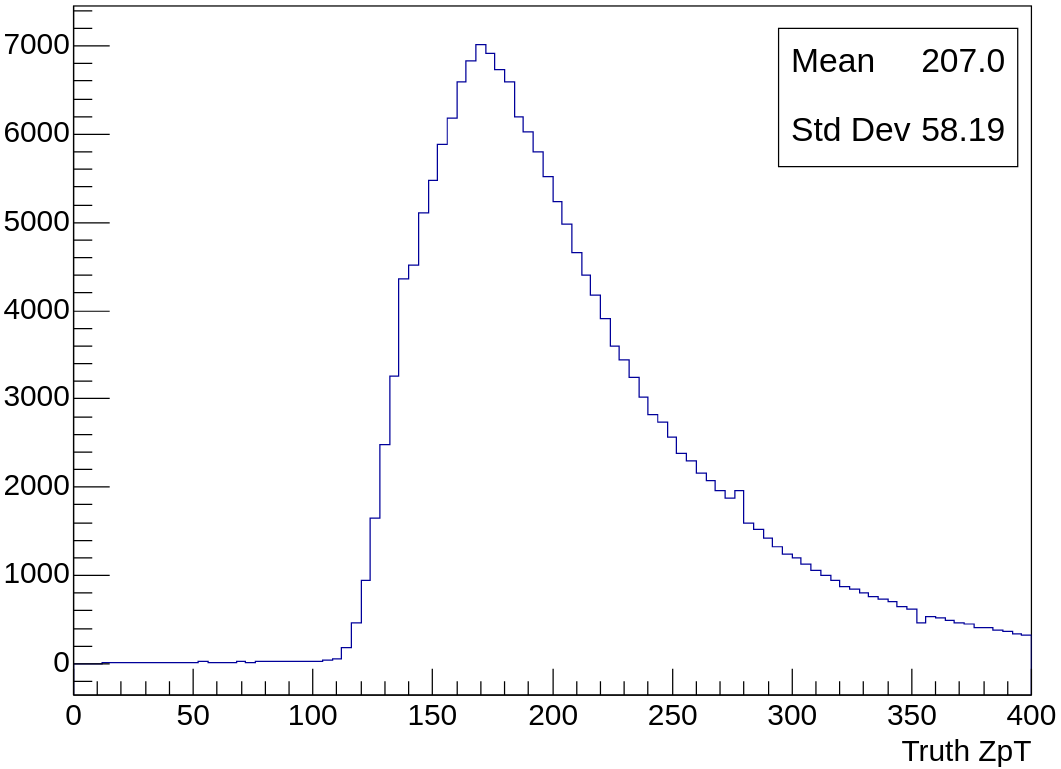
\includegraphics[width=0.50\textwidth]{figures/Fig13d.png}}}
	\subfloat[]{\label{Fig14d}{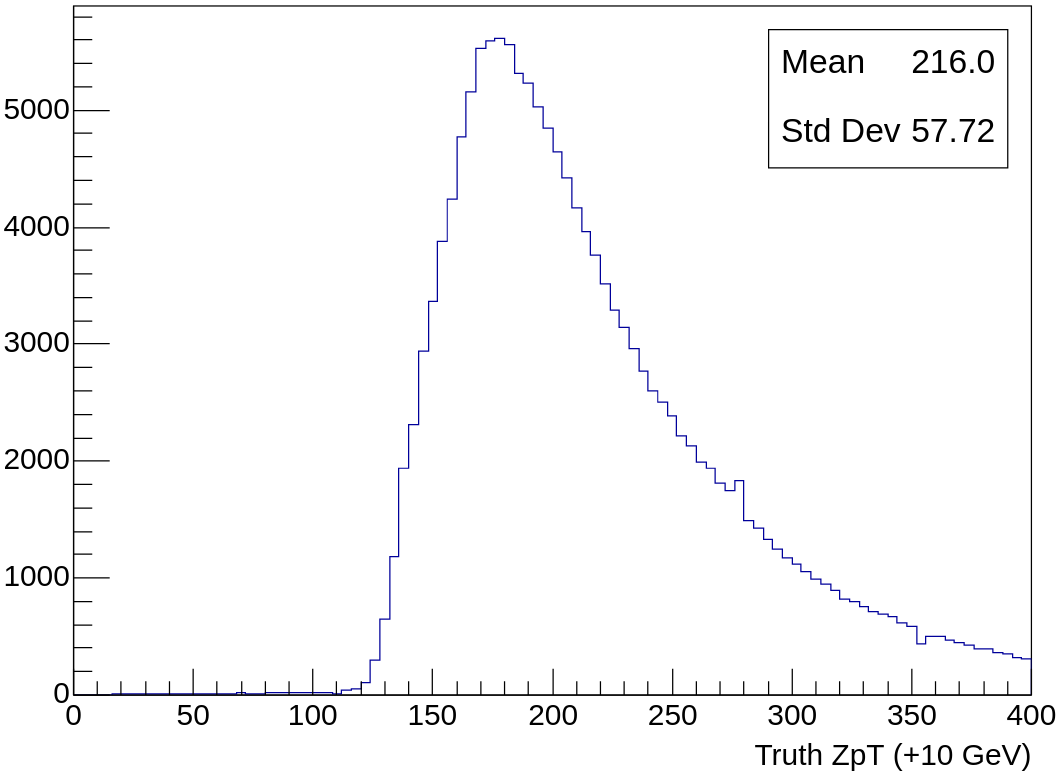
\includegraphics[width=0.50\textwidth]{figures/Fig14c.png}}}
	\caption{Truth Z-$(\pt)$ distributions for different values of the last lepton $\pt$ cut in the $Z\to\mu\mu$ signal sample. (a) -20 GeV selection, (b) -10 GeV selection, (c) standard selection and (d) +10 GeV selection.}
	\label{Fig14}
\end{figure}





